\documentclass{article}

\usepackage[left=2.5cm, right=2.5cm, top=2cm, bottom=2cm]{geometry}

% math mode additions
\usepackage{amsmath}
\usepackage{amsfonts}
\usepackage{amssymb}
\usepackage{physics}
\usepackage{slashed}
\usepackage{mathtools}
% nice 3-vectors
\usepackage{esvect}
% nice differentation
% Get straight d's when differantiating
\usepackage[ISO]{diffcoeff}


% appendix
\usepackage[title]{appendix}
% \usepackage[intlimits]{mathtools}

\usepackage[export]{adjustbox}

% in-document references
\usepackage{hyperref}
\usepackage[capitalize]{cleveref}

% create plots
\usepackage{tikz}
\usepackage[compat=1.1.0]{tikz-feynman}
\usepackage{pgfplots}
\pgfplotsset{compat=1.16}

% Nice table of contents
\usepackage{tocloft}

% Get floats right
\usepackage[section]{placeins}

% adjust fig captions
\usepackage{caption}
\usepackage{subcaption}
\captionsetup{width=.9\textwidth}

\usepackage{titlepic}
% \usepackage[textsize=footnotesize]{todonotes}
\usepackage[disable]{todonotes}

\usepackage[style=numeric-comp,sorting=none,sortcites=true,doi=true,url=false,giveninits=true,hyperref]{biblatex}

\setlength{\marginparwidth}{2.2cm}

\setlength\cftparskip{1pt}
\setlength\cftbeforechapskip{0pt}

\setlength{\parindent}{0em}
\setlength{\parskip}{0.8em}

\def\equationautorefname~#1\null{Eq.~(#1)\null}


% Simple shortcuts
\newcommand{\Ell}{\mathcal{L}}      % Lagrangian L
\newcommand{\He}{\mathcal{H}}       % Hamiltonian H
\newcommand{\Ve}{\mathcal{V}}       % Potential V
\newcommand{\Em}{\mathcal{M}}       % Manifold M
\newcommand{\Ef}{\mathcal{F}}       % Fancy f
\newcommand{\R}{\mathbb{R}}         % Real numbers
\newcommand{\chpt}{$\chi$PT }       % Chiral pertubation theory
\newcommand{\SU}{\mathrm{SU}}       % SU(n)
\newcommand{\eps}{\varepsilon}      % nice epsilon
% \newcommand{\one}{\mathbb{1}}       % Identity
\newcommand{\hc}{\mathrm{h.c.}}     % Hermitian conjugate
\newcommand{\ex}[1]{\expectationvalue{#1}}
\newcommand{\D}{\mathcal{D}}

\newcommand{\one}{\text{\usefont{U}{bbold}{m}{n}1}}
\MakeRobust{\one}

% Big-O notation 
\newcommand{\Oh}[2][2]{\mathcal{O}\left(#2^{#1}\right)}

% (anti) commutator
\newcommand{\com}[2]{\left[#1, #2 \right]}
\newcommand{\acom}[2]{\left\{#1, #2 \right\}}

% Lie algebra
\newcommand{\liea}[2]{\mathfrak{#1}\left(#2\right)}
\newcommand{\lieg}[2]{\mathrm{#1}\left(#2\right)}

% Curly brackets
\newcommand{\C}[1]{\left\{ #1 \right\}}

% Fourier Transform
\newcommand{\F}[1]{\mathcal{F}\C{#1}}
\newcommand{\FInv}[1]{\mathcal{F}^{-1}\C{#1}}

% operator in braket
\newcommand{\inner}[3]{\left\langle #1 {\left| #2 \right|} #3 \right\rangle}

\newcommand{\T}[1]{\textrm{T}_\tau \left\{ #1 \right\}}

% \usepackage{glossaries}

\makenoidxglossaries

\newglossaryentry{chi}
{
    name={$\chi$},
    description={Free parameter in the first order chiral Lagrangian. Related to the mass of the pion}
}


\title{Chiral Perturbation Theory}
\author{Martin Johnsrud}

%%%%%%%%%%%%%%%%%%%%%%%%%%%%%%%%%%%%%%%%%%%%%%%%%%%%%%%
%%%%%%% TODO %%%%%%%
% Forklare hva \alpha er (forstå hva \alpha er)
% være mer konsekevent på parantes {[()]}
% Forklare power counting og effective Lagrangian
% Sjekke partial integraion pi1 d0 pi2
% Nevne at vi ser bort fra WZW-termer
% Referanser i stigende rekkefølge
%%%%%%%%%%%%%%%%%%%%%%%%%%%%%%%%%%%%%%%%%%%%%%%%%%%%%%%

%%%%%%%%%%%%%%%%%%%%%%%%%%%%%%%%%%%%
%%%%%%%%%%%%% SPØRSMÅL %%%%%%%%%%%%%
%%%%%%%%%%%%%%%%%%%%%%%%%%%%%%%%%%%%
% Setter vi faktisk m = 0? Hvordan har vi parameteren \chi hvis m = 0
% Hvordan er SU(2)(kompakt) isomorf til R^3???
% Hvor kommer EOM inn i bildet? Det ser ut som det bare er et navn...
% Kan jeg droppe l_4 termen?
% Lingningsnummer --- når?
% Overskrifter --- Stpr bokstav?
% Hvorfor kan vi bruke EOM fra en annen parametrisering?

%%% Ting og fikse %%%
% Bytt fra \omega til \omega_p/k og bruk det over alt


\begin{document}
\maketitle 

% % Effective Lagrangian
\section{Effective Pion Lagrangian}
The technique used in \chpt to obtain the effective Lagrangian of the pion relies on a ``theorem'', as formulated by Weinberg:
\begin{quote}
    [I]f one writes down the most general possible Lagrangian, including all terms consistent with assumed symmetry principles, and then calculates matrix elements with this Lagrangian to any given order of perturbation theory, the result will simply be the most general possible S-matrix consistent with analyticity, perturbative unitary, cluster decomposition and the assumed symmetry principles. \cite{WeinbergPhenom}
\end{quote}
In other words, if we write down the most general Lagrange density consistent with symmetries of the underlying theory, it will result in the most general S-matrix consistent with that theory, and important physical assumptions.
This leaves a Lagrange density with infinitely many terms, and infinitely many free parameters.
To be able to use this theory for anything one must have a method for ordering the terms in order of importance.
As described in \cite{Scherer2002IntroductionTC}, by rescaling the external momenta $p_\mu \rightarrow t p_\mu$ and quark masses $m_i \rightarrow t^2 m_i$, each term in the Lagrangian obtains a factor $t^D$.
The Lagrangian is then expanded as $\Ell = \sum_D \Ell_D$, where $\Ell_D$ contains all terms with a factor $t^D$.

In our case, the underlying theory is QCD with two quarks, up and down, with mass matrix 
\begin{equation}
    \label{Mass matrix}
    M =
    \begin{pmatrix}
        m_u & 0 \\
        0 & m_d
    \end{pmatrix}.
\end{equation}
In the isospin limit, $m_u = m_d$, the theory is invariant under global transformations by elements of the group $G' = \lieg{SU}{2}_L \times \lieg{SU}{2}_R \times \lieg{U}{1}_V$.
All terms involving only pions are trivially invariant under $\lieg{U}{1}_V$, (HVORFOR?) so we focus on the $G = \lieg{SU}{2}_L \times \lieg{SU}{2}_R$ subgroup.
This symmetry is spontaneously broken if the quark field has a non-zero ground state expectation value $\ex{\bar q q}$, leaving only a subgroup $H = \lieg{SU}{2}_V \subseteq G$ of symmetry transformations of the vacuum state.
The Goldstone manifold $G/H = \lieg{SU}{2}_A$ is a three-dimensional Lie group, and therefore results in three (pseudo) Goldstone bosons, the pions.
There exists an isomorphism from a subset $S \subseteq M_1$ of the set of all Goldstone-fields
\begin{equation*}
    M_1 = \C{ \pi_a: \Em_4 \longrightarrow \R^3 | \pi_a \, \mathrm{smooth} }
\end{equation*}
close to the ground state, into fields taking values in the Goldstone manifold $G/H$. (BEVISE?)(HVA ER ISOMORFISME HER?).
The \chpt effective Lagrangian will be constructed using this map, through the parametrization
\begin{align}
\label{sigma}
    \Sigma : \Em_4 & \longrightarrow \lieg{SU}{2},\\ \notag
    x & \longrightarrow \Sigma(x) = A_\alpha (U(x) \Sigma_0 U(x)) A_\alpha,
\end{align}
where
\begin{align*}
    \Sigma_0 = \one,\, 
    A_\alpha = \exp(\frac{i \alpha}{2} \tau_1),\, 
    U(x) = \exp(i \frac{\tau_a\pi_a(x)}{2f}).
\end{align*}
$\tau_a$ are the $\SU(2)$ generators, i.e. Pauli matrices, as described in \autoref{Conventions and notation}.
$\pi_a$, where $ \, a \in \C{1, 2, 3}$, are the pion fields. These are real fields, meaning $\pi_a^\dagger = \pi_a$.

% Veldig uferdig. Trenger teori om Goldstones theorem
\section{Leading order Lagrangian}

The leading order \chpt Lagrangian is made up of the terms \cref{leading order chi sigma term} and \cref{leading order term sigma}, and reads
\begin{equation}
    \label{chpt lagrangian}
    \Ell_2 = 
    \frac{1}{4} f^2 \Tr{\nabla_\mu \Sigma (\nabla^\mu \Sigma)^\dagger}
    + \frac{1}{4} f^2 \Tr{\chi^\dagger \Sigma + \Sigma^\dagger \chi}.
\end{equation}
In the ground state, we set the external scalar current $s = m$, where $m$ is the mass matrix \autoref{Mass matrix}, so
\begin{equation}
    \chi = 2 B_0 m = \bar m^2 \one + \Delta m^2 \tau_3,
\end{equation}
where we have defined
\begin{equation}
    \bar m^2 = B_0(m_u + m_d), \quad \Delta m^2 = B_0 (m_u - m_d).
\end{equation}
In this section, we will expand this Lagrangian in $\pi/f$, which we will use to calculate the free energy density.
To get the series expansion of $\Sigma$ in powers of $\pi/f$, we start by using the fact that $\tau_a^2 = \one$ to write
\begin{equation}
    \label{A}
    A_\alpha 
    = \sum_n^\infty \frac{1}{n!} \left(\frac{i \alpha}{2} \tau_1 \right)^n 
    = \sum_n^\infty 
    \left[
        \frac{\one}{(2n)!} \left(\frac{i \alpha}{2}\right)^{(2n)} 
        + \frac{\tau_1}{(2n + 1)!} \left(\frac{i\alpha}{2}\right)^{(2n + 1)}
    \right] 
    = \one \cos{\frac{\alpha}{2}} + i \tau_1 \sin{\frac{\alpha}{2}}.
\end{equation}
The series expansion of $U$ is
\begin{align*}
    U = \exp(\frac{i \pi_a \tau_a}{2f}) = 
    1
    + \frac{i \pi_a \tau_a}{2f} 
    + \frac{1}{2}\left(\frac{i \pi_a \tau_a}{2f}\right)^2 
    + \frac{1}{6}\left(\frac{i \pi_a \tau_a}{2f}\right)^3 
    + \frac{1}{24}\left(\frac{i \pi_a \tau_a}{2f}\right)^4 
    + \Oh[5]{(\pi/f)},
\end{align*}
which we use to calculate the expansion of the inner part of $\Sigma$, as given in \autoref{sigma},
\begin{align*}
    U\Sigma_0U & = 
    \left(
        1
        + \frac{i \pi_a \tau_a}{2f} 
        + \frac{1}{2}\left(\frac{i \pi_a \tau_a}{2f}\right)^2 
        + \frac{1}{6}\left(\frac{i \pi_a \tau_a}{2f}\right)^3 
        + \frac{1}{24}\left(\frac{i \pi_a \tau_a}{2f}\right)^4 
    \right)\\
    & \times
    \left(
        1
        + \frac{i \pi_a \tau_a}{2f} 
        + \frac{1}{2}\left(\frac{i \pi_a \tau_a}{2f}\right)^2 
        + \frac{1}{6}\left(\frac{i \pi_a \tau_a}{2f}\right)^3 
        + \frac{1}{24}\left(\frac{i \pi_a \tau_a}{2f}\right)^4 
    \right)
    + \Oh[5]{(\pi/f)}\\
    &=
    1 + \frac{i \pi_a \tau_a}{f}
    + 2 \left( \frac{i \pi_a \tau_a}{2f} \right)^2
    + \frac{4}{3} \left( \frac{i \pi_a \tau_a}{2f} \right)^3
    + \frac{2}{3} \left( \frac{i \pi_a \tau_a}{2f} \right)^4
    + \Oh[5]{(\pi/f)}.
\end{align*}
The symmetry of $\pi_a\pi_b$ means that
\begin{align*}
% Identitites
    & (\pi_a \tau_a)^2
    = 
    \pi_a \pi_b \frac{1}{2} \acom{\tau_a}{\tau_b} 
    =
    \pi_a \pi_a, \quad
    (\pi_a \tau_a)^3
    =
    \pi_a \pi_a \pi_b \tau_b,\quad
    (\pi_a \tau_a)^4
    =
    \pi_a \pi_a \pi_b \pi_b.
\end{align*}
This gives us the expression
\begin{align*}
% Final expression
    & U\Sigma_0U 
    =
    1
    + i \frac{\pi_a \tau_a}{f} 
    - \frac{\pi_a^2}{2f^2}
    - i \frac{\pi_a^2\pi_b \tau_b}{6f^3}
    + \frac{\pi_a^2\pi_b^2}{24f^4}
    + \Oh[5]{(\pi/f)}.
\end{align*}
We combine this result with \autoref{A} to get an expression for $\Sigma$ up to $\Oh[5]{(\pi/f)}$
\begin{align*}
    \Sigma 
    % & =   
    % \Big( \cos{\frac{\alpha}{2}} + i \tau_1 \sin{\frac{\alpha}{2}} \Big) 
    % \left(
    %     1
    %     + i \frac{\pi_a \tau_a}{f} 
    %     - \frac{\pi_a^2}{2f^2}
    %     - i \frac{\pi_a^2\pi_b \tau_b}{6f^3}
    %     + \frac{\pi_a^2\pi_b^2}{24f^4}    
    % \right)
    % \Big( \cos{\frac{\alpha}{2}} + i \tau_1 \sin{\frac{\alpha}{2}} \Big) \\
    & =
    \left(
        1
        + i \frac{\pi_a \tau_a}{f} 
        - \frac{\pi_a^2}{2f^2}
        - i \frac{\pi_a^2\pi_b \tau_b}{6f^3}
        + \frac{\pi_a^2\pi_b^2}{24f^4}    
    \right)
    \cos^2{\frac{\alpha}{2}} \\
    & -
    \left(
        1
        + i \frac{\pi_a}{f} \tau_1\tau_a\tau_1
        - \frac{\pi_a^2}{2f^2}
        - i \frac{\pi_a^2\pi_b}{6f^3} \tau_1\tau_b\tau_1
        + \frac{\pi_a^2\pi_b^2}{24f^4}
    \right)
    \sin^2{\frac{\alpha}{2}}\\
    & + i
    \left(
        2 \tau_1
        + i \frac{\pi_a}{f} \acom{\tau_1}{\tau_a}
        - 2\tau_1 \frac{\pi_a^2}{2f^2}
        - i \frac{\pi_a^2\pi_b}{6f^3} \acom{\tau_1}{\tau_b}
        + 2\tau_1 \frac{\pi_a^2\pi_b^2}{24f^4}
    \right)
    \sin{\frac{\alpha}{2}}\cos{\frac{\alpha}{2}}.
\end{align*}
Using trigonometric identities and the commutator,
\begin{align*}
    \cos^2{\frac{\alpha}{2}} - \sin^2{\frac{\alpha}{2}} = \cos{\alpha}, \quad 
    2 \cos{\frac{\alpha}{2}} \sin{\frac{\alpha}{2}} = \sin{\frac{\alpha}{2}}, \quad
    \tau_1 \tau_a \tau_1
    = -\tau_a + 2 \delta_{1a}\tau_1,
\end{align*}
the final expression of $\Sigma$ to $\Oh[5]{(\pi/f)}$ is
\begin{align}
    \Sigma =
     \left(
        1 
        - \frac{\pi_a^2}{2f^2}
        + \frac{\pi_a^2\pi_b^2}{24f^4}
    \right)
    (\cos{\alpha} + i \tau_1 \sin{\alpha})
    +
    \left(
        \frac{\pi_a}{f} 
        - \frac{\pi_b^2\pi_a}{6f^3} 
    \right)
    \left(
        i\tau_a - 2i \delta_{a1}\tau_1\sin^2{\frac{\alpha}{2}} - \delta_{a1} \sin{\alpha}
    \right).
    \label{expansion of sigma}
\end{align}

The kinetic term in the \chpt Lagrangian is
\begin{equation}
    \nabla_\mu \Sigma (\nabla^\mu \Sigma)^\dagger 
    = \partial_\mu \Sigma \partial^\mu \Sigma^\dagger 
    - i \left(\partial_\mu \Sigma \com{v^\mu}{\Sigma^\dagger} - \hc \right)
    - \com{v_\mu}{\Sigma}\com{v_\mu}{\Sigma^\dagger}.
    \label{kinetic term}
\end{equation}
Using \autoref{expansion of sigma} we find the expansion of the constitutive parts of the kinetic term to be
\begin{align}
    \notag
    \partial_\mu \Sigma 
    = &
    % \left(
    %     \frac{-1}{f^2}
    %     + \frac{\pi_b^2}{6f^4}
    % \right)
    % (\cos{\alpha} + i \tau_1 \sin{\alpha}) (\pi_a \partial_\mu \pi_a)\\\notag
    % +&
    % \left(
    %     \frac{\partial_\mu \pi_a}{f} 
    %     - \frac{\pi_b^2 \partial_\mu\pi_a 
    %     + 2 \pi_a \pi_b \partial_\mu\pi_b}{6f^3} 
    % \right)
    % \left(
    %     i\tau_a - 2i \delta_{a1}\tau_1\sin^2{\frac{\alpha}{2}} - \delta_{1a} \sin{\alpha}
    % \right)
    % \\ \notag
    % =& 
    \left[
        \left(
            \frac{-1}{f^2}
            + \frac{\pi_b^2}{6f^4}
        \right)
        (\pi_a \partial_\mu \pi_a)
        \cos{\alpha}
        - 
        \left(
            \frac{\partial_\mu \pi_1}{f} 
            - \frac{\pi_b^2 \partial_\mu\pi_1
            + 2 \pi_1 \pi_b \partial_\mu\pi_b}{6f^3} 
        \right)
        \sin{\alpha}
    \right]
    \\ \notag 
    - &
    \left[
        \left(
            \frac{-1}{f^2}
            + \frac{\pi_b^2}{6f^4}
        \right)
        (\pi_a \partial_\mu \pi_a)
        \sin{\alpha}
        - \left(
        \frac{\partial_\mu \pi_1}{f} 
        - \frac{\pi_b^2 \partial_\mu\pi_1
        + 2 \pi_1 \pi_b \partial_\mu\pi_b}{6f^3}
        \right)
        2 \sin^2{\frac{\alpha}{2}}
    \right]
    i \tau_1 \\ \label{Sigma derivative}
    +& 
    \left(
        \frac{\partial_\mu \pi_a}{f} 
        - \frac{\pi_b^2 \partial_\mu\pi_a 
        + 2 \pi_a \pi_b \partial_\mu\pi_b}{6f^3} 
    \right)
    i \tau_a,
\end{align}
and
\begin{align}
    % \notag
    \com{v_\mu}{\Sigma} 
    % & = 
    % \frac{1}{2} \mu_I \delta^0_\mu
    % \left[
    %     \left(
    %         1 
    %         - \frac{\pi_a^2}{2f^2}
    %         + \frac{\pi_a^2\pi_b^2}{24f^4}
    %     \right)
    %     i \sin{\alpha} \com{\tau_3}{\tau_1}
    %     + 
    %     \left(
    %         \frac{\pi_a}{f} 
    %         - \frac{\pi_b^2\pi_a}{6f^3} 
    %     \right)
    %     \left(
    %         i\com{\tau_a}{\tau_3} 
    %         - 2i\delta_{a1}\sin^2{\frac{\alpha}{2}}\com{\tau_3}{\tau_1}
    %     \right)
    % \right] \\
    % \notag
    % & =
    % -\mu_I \delta^0_\mu
    % \left\{
    %     \left(
    %         1 
    %         - \frac{\pi_a^2}{2f^2}
    %         + \frac{\pi_a^2\pi_b^2}{24f^4}
    %     \right)
    %     \tau_2 \sin{\alpha}
    %     + 
    %     \left(
    %         \frac{\pi_a}{f} 
    %         - \frac{\pi_b^2\pi_a}{6f^3} 
    %     \right)
    %     \left[
    %         (\delta_{a1} \tau_2 - \delta_{a2} \tau_1)
    %         - 2\delta_{a1} \tau_2 \sin^2{\frac{\alpha}{2}}
    %     \right]
    % \right\} \\
    & =
    -\mu_I \delta^0_\mu
    \left\{
        \left[
        \left(
            1 
            - \frac{\pi_a^2}{2f^2}
            + \frac{\pi_a^2\pi_b^2}{24f^4}
        \right)
        \sin{\alpha}
        + 
        \left(
            \frac{\pi_1}{f} 
            - \frac{\pi_b^2\pi_1}{6f^3} 
        \right) \cos{\alpha}
        \right]
         \tau_2
        -
        \left(
            \frac{\pi_2}{f} 
            - \frac{\pi_b^2\pi_2}{6f^3} 
        \right)
        \tau_1
    \right\}.
    \label{sigma commutator}
\end{align}
Combining \autoref{Sigma derivative} and \autoref{sigma commutator} gives the following terms \footnote{The scripts used to aid the calculation of the Lagrangian is available at \url{https://github.com/martkjoh/prosjektopggave}}
\begin{align*}
    % Term 1
    & \Tr{\partial_\mu \Sigma \partial^\mu \Sigma^\dagger}
    = \frac{2}{f^2} \partial_\mu \pi_a \partial^\mu \pi_a
    + \frac{2}{3f^4}
    \left[
        (\pi_a\partial_\mu \pi_a)(\pi_b\partial^\mu \pi_b)
        -        
        (\pi_a\partial_\mu \pi_b)(\pi_b\partial^\mu \pi_a)
    \right], \\
    % Term 2
    -i  &\Tr{\partial^\mu\Sigma\com{v_\mu}{\Sigma^\dagger} - \hc}
    =
    4 \mu_I \frac{\partial_0\pi_2}{f}
    + 8 \mu_I \frac{\pi_3}{3f^3}\sin{\alpha}(
        \pi_2 \partial_0 \pi_3 - \pi_3 \partial_0 \pi_2
        ) \sin{\alpha}
    \\ & \quad \quad \quad \quad \quad \quad \quad \quad \quad \quad \quad
    +
    \left(
        \frac{4\mu_I}{f^2} \cos{\alpha}
        - \frac{8 \mu_I\pi_1}{3f^3} \sin{\alpha}
        - \frac{4 \mu_I \pi_a \pi_a} {3f^4}\cos{\alpha} 
    \right) 
    (\pi_1\partial_0 \pi_2 - \pi_2 \partial_0 \pi_1), \\
    % Term 3
    - & \Tr{\com{v_\mu}{\Sigma}\com{v^\mu}{\Sigma^\dagger}}
    = \mu_I{}^2
    \bigg[
        2 \sin^2{\alpha}
        +
        \left(
            \frac{2}{f} 
            - \frac{4\pi_a \pi_a}{3 f^3} 
        \right)
        \pi_1  \sin{2\alpha}
        + \left(
            \frac{2}{f^2}
            - \frac{2 \pi_a \pi_a}{3 f^4} 
        \right)
        \pi_a \pi_b k_{ab}
    \bigg], 
    \\
    % Mass Term
    & \Tr{\chi^\dagger \Sigma + \Sigma^\dagger\chi}
    = 
    \bar m^2 
    \left(
        4 \cos{\alpha} 
        - \frac{4 \pi_1}{f} \sin{\alpha} 
        - \frac{2 \pi_a \pi_a}{f^2} \cos{\alpha}
        + \frac{2 \pi_1 \pi_a \pi_a}{3 f^3} \sin{\alpha}
        + \frac{(\pi_a \pi_a)^2}{6 f^4}\cos{\alpha}
    \right), 
    \end{align*}
where $k_{ab} =\delta_{a1} \delta_{b1} \cos{2\alpha}  + \delta_{a2}\delta_{b2}\cos^2{\alpha} - \delta_{a3}\delta_{b3} \sin^2{\alpha}$.
Notice that the mass term is independent of the difference in quark masses, $\Delta m$.
If we write the Lagrangian as show in \autoref{chpt lagrangian} as $\Ell_2 = \Ell_2^{(0)} + \Ell_2^{(1)} + \Ell_2^{(2)} +...$, where $\Ell_2^{(n)}$ contains all terms of order $\Oh[n]{(\pi/f)}$, then the result of the series expansion is
\begin{align}
%%%%%%%%%%%%%%%%%%
%% zeroth order %%
%%%%%%%%%%%%%%%%%%
\Ell_2^{(0)}
&  =
    f^2   
    \left(
        \bar m^2 \cos{\alpha}
        + \frac{1}{2} \mu^2 \sin^2{\alpha}
    \right),
    \label{L0}
\\
%%%%%%%%%%%%%%%%%%
%% first order %%
%%%%%%%%%%%%%%%%%%
\label{L1}
\Ell_2^{(1)}
& =
    f 
    (
        \mu_I^2\cos{\alpha}
        - \bar m^2
    ) \pi_1 \sin{\alpha}
    + f \mu_I \partial_0\pi_2 \sin{\alpha},
\\
%%%%%%%%%%%%%%%%%%
%% second order %%
%%%%%%%%%%%%%%%%%%
\Ell_2^{(2)}
& =
    \frac{1}{2} \partial_\mu\pi_a\partial^\mu\pi_a
    + \mu_I \cos{\alpha} \left( \pi_1 \partial_0\pi_2 - \pi_2\partial_0\pi_1 \right)
    - \frac{1}{2} \bar m^2 \pi_a \pi_a \cos{\alpha}
    + \frac{1}{2} \mu_I ^2 \pi_a \pi_b k_{ab},
\label{L2}
\\
%%%%%%%%%%%%%%%%%%
%% third order %%
%%%%%%%%%%%%%%%%%%
\notag
\Ell_2^{(3)}
& =
    \frac{\pi_a\pi_a \pi_1}{6f}
    (\bar m^2 \sin{\alpha}-2\mu_I{}^2 \sin{2\alpha})\\ \label{L3}
    &
    -
    \frac{2 \mu_I}{3 f}
    \left[
        \pi_1(\pi_1 \partial_0\pi_2 - \pi_2\partial_0\pi_1)
        +
        \pi_3(\pi_3\partial_0\pi_2-\pi_2 \partial_0\pi_3)
    \right]
    \sin{\alpha},
\\
%%%%%%%%%%%%%%%%%%
%% fourth order %%
%%%%%%%%%%%%%%%%%%
\notag
\Ell_2^{(4)}
& =
\frac{1}{6f^2}
\curly{    
    \frac{1}{4} \bar m^2 (\pi_a\pi_a)^2 \cos{\alpha}
    -
    \left[
        (\pi_a \pi_a) (\partial_\mu \pi_b \partial^\mu \pi_b )
        - (\pi_a \partial_\mu \pi_a)(\pi_b \partial^\mu \pi_b )
    \right]
}
\\
&
- \frac{\mu_I \pi_a\pi_a}{3f^2}
\left[
    \left(\pi_1\partial_0 \pi_2 - \pi_2 \partial_0 \pi_1\right)
    \cos{\alpha}
    + \frac{1}{2} \mu_I \pi_a \pi_b k_{ab}
\right].
\label{L4}
\end{align}

% For det meste ferdig
\section{Equation of motion and redundant terms}

Changing the field parametrization that appear in the Lagrangian does not affect any of the physics, as it corresponds to a change of variables in the path integral~\cite{Scherer2002IntroductionTC,Chisholm:changeOfVar,Kamefuchi:changeOfVar}.
However, a change of variables can result in new terms in the Lagrangian.
As a result of this, terms that on the face of it appear independent may be redundant.
These terms can be eliminated by using the classical equation of motion.
In this section we show first the derivation of the equation of motion, then use this result to identify redundant terms which need not be included in the most general Lagrangian.

We derive the equation of motion for the leading order Lagrangian using the principle of least action.
Choosing the parametrization $\Sigma = \exp(i \pi_a \tau_a)$, a variation $\pi_a \rightarrow \pi_a + \delta \pi_a$ results in a variation in $\Sigma$, $\delta \Sigma = i \tau_a \delta \pi_a \Sigma $.
The variation of the leading order action,
\begin{equation}
    S_2 = \int_\Omega \dd^4x \, \Ell_2,
\end{equation}
when varying $\pi_a$ is 
\begin{align*}
    \delta S = \int_\Omega \dd x \, \frac{f^2}{4}
    \Tr{
        (\nabla_\mu \delta \Sigma) (\nabla^\mu \Sigma)^\dagger
        + (\nabla_\mu \Sigma) (\nabla^\mu \delta \Sigma)^\dagger
        + \chi \delta \Sigma^\dagger + \delta \Sigma \chi^\dagger
    }.
\end{align*}
Using the properties of the covariant derivative to do partial integration, as show in \autoref{Covarinat derivative}, as well as $\delta(\Sigma \Sigma^\dagger) = (\delta\Sigma)\Sigma^\dagger + \Sigma (\delta \Sigma)^\dagger = 0$, the variation of the action can be written
\begin{align*}
    \delta S 
    & = \frac{f^2}{4} \int_\Omega \dd x\, 
    \Tr{
        - \delta \Sigma \nabla^2 \Sigma^\dagger
        + (\nabla^2 \Sigma) (\Sigma^\dagger \delta \Sigma \Sigma^\dagger)
        - \chi (\Sigma^\dagger \delta \Sigma \Sigma^\dagger)
        + \delta \Sigma \chi^\dagger
    } \\
    & = 
    \frac{f^2}{4} \int_\Omega \dd x\, 
    \Tr{
        \delta \Sigma \Sigma^\dagger 
        \left[
            (\nabla^2 \Sigma)\Sigma^\dagger
            - \Sigma \nabla^2 \Sigma^\dagger
            - \chi \Sigma^\dagger
            + \Sigma \chi^\dagger
        \right]
        } \\
    & = 
    i \frac{f^2}{4} \int_\Omega \dd x\, 
    \Tr{\tau_a 
    \left[
         (\nabla^2 \Sigma)\Sigma^\dagger
        - \Sigma \nabla^2 \Sigma^\dagger
        - \chi \Sigma^\dagger
        + \Sigma \chi^\dagger
    \right]
    } 
    \delta \pi_a = 0.
\end{align*}  
As the variation is arbitrary, the equation of motion to leading order is
\begin{equation}
    \Tr{
        \tau_a 
        \left[
            (\nabla^2 \Sigma)\Sigma^\dagger
            - \Sigma \nabla^2 \Sigma^\dagger
            - \chi \Sigma^\dagger
            + \Sigma \chi^\dagger
        \right]
    } = 0.
\end{equation}
We define
\begin{equation}
    \mathcal O_\text{EOM}^{(2)}
    = 
    (\nabla^2 \Sigma)\Sigma^\dagger
    - \Sigma \nabla^2 \Sigma^\dagger
    - \chi \Sigma^\dagger
    + \Sigma \chi^\dagger.
\end{equation}
% This may be rewritten as a matrix equation. 
% Using that 
% \begin{align*}
%     \Tr{(\nabla_\mu \Sigma)\Sigma^\dagger}
%     = 
%     \Tr{i \tau_a (\partial_\mu \pi_a )\Sigma \Sigma^\dagger}
%     - i\Tr{[v_\mu, \Sigma]\Sigma^\dagger}
%     = 0,
% \end{align*}
% we can see that $\Tr{(\nabla^2 \Sigma)\Sigma^\dagger - \Sigma \nabla^2 \Sigma^\dagger} = 0$, and the equation of motion may be written as
% \begin{equation}
%     \label{EOM matrix form}
%     \mathcal{O}_\mathrm{EOM}^{(2)}(\Sigma) 
%     = 
%     (\nabla^2 \Sigma)\Sigma^\dagger
%     - \Sigma \nabla^2 \Sigma^\dagger
%     - \chi \Sigma^\dagger
%     + \Sigma \chi^\dagger
%     - \frac{1}{2}
%     \Tr{ \chi \Sigma^\dagger - \Sigma \chi^\dagger} = 0.
% \end{equation}

The next step in eliminating redundant terms is to change the parametrization of $\Sigma$ by $\Sigma(x) \rightarrow \Sigma'(x)$.
Here, $ \Sigma(x) = e^{iS(x)} \Sigma'(x), \, S(x) \in \liea{su}{2}$. This change leads to a new Lagrange density, $\Ell[\Sigma] = \Ell[\Sigma'] + \Delta \Ell[\Sigma']$.
We are free to choose $S(x)$, as long $\Sigma'$ still obeys the required transformation properties.
Any terms in the Lagrangian $\Delta \Ell$ due to a reparametrization can be neglected, as argued earlier.
When demanding that $\Sigma'$ obey the same symmetries as $\Sigma$,
the most general transformation to second order in Weinberg's power counting scheme  is~\cite{Scherer2002IntroductionTC}
\begin{equation}
    \label{S reparametrization}
    S_{2} = 
    i \alpha_2 
    \left[
        (\nabla^2 \Sigma') \Sigma^\dagger - \Sigma' (\nabla^2 {\Sigma'})^\dagger
    \right]
    + i \alpha_2
    \left[
        \chi \Sigma'^\dagger - \Sigma' \chi^\dagger 
        - \frac{1}{2} \Tr{\chi \Sigma'^\dagger - \Sigma' \chi^\dagger}
    \right].
\end{equation}
$\alpha_1$ and $\alpha_2$ are arbitrary real numbers. As \autoref{S reparametrization} is to second order, $\Delta \Ell$ is fourth order in Weinberg's power counting scheme.
To leading order is given by
\begin{align*}
    \Ell_2\left[e^{i S_2}\Sigma '\right]
    & =
    \frac{f^2}{4}\Tr{[\nabla_\mu (1 +i S_2)\Sigma'][\nabla^\mu \Sigma'^\dagger  (1 - i S_2)]}
    + \frac{f^2}{4} \Tr{\chi\Sigma'^\dagger (1 - i S_2) + (1 +i S_2)\Sigma' \chi^\dagger} \\
    & = \Ell[\Sigma'] + 
    i \frac{f^2}{4}
    \Tr{[\nabla_\mu (S_2\Sigma')][\nabla^\mu\Sigma']^\dagger 
    -  [\nabla_\mu\Sigma'][\nabla^\mu (\Sigma'^\dagger  S_2) ]}
    - i \frac{f^2}{4} \Tr{\chi \Sigma'^\dagger S_2 - S_2 \Sigma' \chi^\dagger}
\end{align*}
Using the properties of the covariant derivative, we may use the product rule and partial integration to write the difference between the two Lagrangians to fourth order as
\begin{align}
    \nonumber
    \Delta \Ell[\Sigma'] 
    & = 
    i \frac{f^2}{4}
    \Tr{
        (\nabla_\mu S_2)
        (\Sigma' \nabla^\mu \Sigma'^\dagger - (\nabla^\mu \Sigma') \Sigma'^\dagger) 
    }
    - i \frac{f^2}{4} \Tr{\chi \Sigma'^\dagger  S_2 - S_2 \Sigma' \chi^\dagger} \\
    & = 
    % i \frac{f^2}{4}
    % \Tr{
    %     S_2
    %     \left[
    %         \Sigma'^\dagger\nabla^2 \Sigma' - ( \nabla^2 \Sigma') \Sigma'^\dagger 
    %         - \chi\Sigma'^\dagger + \Sigma' \chi^\dagger
    %     \right]
    % }
    \label{Delta reparametrization}
    \frac{f^2}{4} \Tr{i S_2 \mathcal{O}_\mathrm{EOM}^{(2)}}.
\end{align}
Any term that can be written in the form of \autoref{Delta reparametrization} for arbitrary $\alpha_1, \alpha_2 \in \R$ is redundant, as we argued earlier, and may therefore be discarded.
$\Delta \Ell_2$ is of fourth order, and it can thus be used to remove terms from $\Ell_4$ or higher order.

% Ikke ferdig. Se på mer senere
\subsection{Next to leading order Lagrangian}

The next to leading order Lagrangian density is, assuming no external fields
\begin{align}
    \notag
    \Ell_4 
    & = 
    \frac{l_1}{4} \Tr{\nabla_\mu \Sigma (\nabla^\mu \Sigma)^\dagger}^2
    + \frac{l_2}{4} \Tr{\nabla_\mu \Sigma (\nabla_\nu \Sigma)^\dagger} 
    \Tr{\nabla^\mu \Sigma (\nabla^\nu \Sigma)^\dagger} 
    +
    \frac{l_3 + h_1 - h_3 }{16} \Tr{\chi \Sigma^\dagger + \Sigma \chi^\dagger}^2
    \\ \notag
    &
    + \frac{l_4}{4}\Tr{\nabla_\mu \Sigma (\nabla^\mu \Sigma)^\dagger} \Tr{\chi \Sigma^\dagger + \Sigma \chi^\dagger}
    + \frac{h_1 - h_3 - l_4-l_7}{16} \Tr{\chi \Sigma^\dagger - \Sigma \chi^\dagger}^2
    + \frac{h_1 + h_2 - l_4}{4} \Tr{\chi \chi^\dagger} \\
    & -
    \frac{h_1 - h_3 - l_4}{8} 
        \Tr{\left(\chi \Sigma^\dagger\right)^2 + \left( \Sigma \chi^\dagger\right)^2}
    \label{NLO Lagrangian}
\end{align}
 
To $\Ell_4$ to $\Oh[3]{(\pi/f)}$, we use the result from \autoref{Sigma derivative} and \autoref{sigma commutator},
% \begin{align*}
%     \Sigma & =
%     \left(
%        1 
%        - \frac{\pi_a^2}{2f^2}
%    \right)
%    (\cos{\alpha} + i \tau_1 \sin{\alpha})
%    +  \frac{\pi_a}{f}
%    \left(
%        i\tau_a 
%        - 2i \delta_{a1} \tau_1 \sin^2{\frac{\alpha}{2}}
%        - \delta_{a1} \sin{\alpha}
%    \right), \\
%     \partial_\mu \Sigma 
%     & = 
%     - \frac{\pi_a \partial_\mu \pi_a}{f^2}
%     \left(\cos{\alpha} + i \tau_1 \sin{\alpha}\right)
%     + \frac{\partial_\mu \pi_a}{f}
%     \left(
%         i\tau_a 
%         -2 i \delta_{a1} \tau_1 \sin^2{\frac{\alpha}{2}}
%         - \delta_{a1}\sin{\alpha}\right), \\
%     [v_\mu, \Sigma^\dagger] 
%     & =
%     \mu_I \delta^0_\mu
%     \left[
%         \left( 1 - \frac{\pi_a^2}{2f^2} \right) \tau_2 \sin{\alpha}
%         + \frac{\pi_a}{f}
%         \left(
%             \delta_{a1} \cos{\alpha} \tau_2 - \delta_{a2} \tau_1
%         \right)
%     \right].
%     \end{align*}
up to and including $\Oh{(\pi/f)}$, which gives
\begin{align*}
    %%%%%%%%%%%%%%%%%%
    % parital square %
    %%%%%%%%%%%%%%%%%%
    \Tr{\partial_\mu \Sigma \partial_\nu \Sigma^\dagger}
    & = 2 \frac{\partial_\mu \pi_a \partial_\nu \pi_a}{f^2} \\
    %%%%%%%%%%%%%%
    % Cross term %
    %%%%%%%%%%%%%
    -i \Tr{\partial_\mu \Sigma \com{v_\nu}{\Sigma^\dagger} - \hc}
    & = 
    \frac{2\mu_I\pi_2}{f}(\delta_\mu^0\partial_\nu + \delta_\nu^0\partial_\mu)\sin{\alpha} + 
    \frac{2\mu_I}{f^2}
    [
        \pi_1 (\delta_\mu^0\partial_\nu + \delta_\nu^0\partial_\mu)\pi_2 
        - \pi_2 (\delta_\mu^0\partial_\nu + \delta_\nu^0\partial_\mu)\pi_1
    ]\cos{\alpha}
    \\
    %%%%%%%%%%%%%%%%%
    % Comm. squared %
    %%%%%%%%%%%%%%%%%
    - \Tr{\com{v_\nu}{\Sigma} \com{v_\nu}{\Sigma^\dagger}}
    & = 2 \mu_I{}^2 \delta_\mu^0 \delta_\nu^0 
    \left[
        \sin^2{\alpha} + \frac{\pi_1}{f} \sin{2\alpha} 
        + \frac{\pi_a \pi_b}{f^2} 
        k_{ab}
    \right].
\end{align*}
Using the form of the Pauli matrices, we can write $\chi$ as 
\begin{align*}
    \chi = 2 B_0 M = 2 B_0 (\bar m \one + \Delta m \tau_3),
\end{align*}
where $\bar m  = (m_u + m_d)/2, \, \Delta m = (m_u - m_d)/2$, which gives 
\begin{align*}
    \chi \Sigma^\dagger + \Sigma \chi^\dagger
    & = 4 B_0 \Bigg\{
         (\bar m + \Delta m \tau_3)
        \left[
            \left(
                1 
                - \frac{\pi_a^2}{2f^2}
            \right)
            \cos{\alpha}
            - \frac{\pi_1}{f}    
            \sin{\alpha}
        \right]\\
    & \quad \quad \quad
    + \Delta m 
    \left[
        \left(
            1 
            - \frac{\pi_a^2}{2f^2}
        \right)
        \tau_2 \sin{\alpha}
        +  \frac{\pi_a}{f}
        \left(
            \delta_{a1} \tau_2 \cos{\alpha} - \delta_{a2} \tau_1
        \right)
    \right]
    \Bigg\}, \\
    %%%%%%%%%%%%%%
    % Difference %
    %%%%%%%%%%%%%%
    \chi \Sigma^\dagger  - \Sigma \chi^\dagger
    & = - 4 i B_0 \Bigg\{
        \bar m 
        \left[
            \left(
                1 - \frac{\pi_a^2}{2f^2}
            \right)
            \tau_1 \sin{\alpha}
            +  \frac{\pi_a}{f}    \left(
                \tau_a 
                - 2 \delta_{1a} \tau_1 \sin^2{\frac{\alpha}{2}}
            \right)        
        \right]
        + \Delta m 
            \frac{\pi_3}{f}
    \Bigg\}.
\end{align*}
Combining these results gives all the terms in $\Ell_4$, to $\Oh[3]{(\pi/f)}$:
%%%%%%%%%%%%%%%%%
% Parts for L_4 %
%%%%%%%%%%%%%%%%%
\begingroup
\allowdisplaybreaks % Make page break possible
\begin{align}
    %%%%%%%
    % l_1 %
    %%%%%%%
    \notag
    & \Tr{\nabla_\mu \Sigma (\nabla^\mu \Sigma)^\dagger}^2 
    =
    \Tr{\partial_\mu \Sigma \partial^\mu \Sigma ^\dagger
    - i \left( \partial_\mu \Sigma \com{v^\mu}{\Sigma^\dagger} - \hc \right)
    - \com{v_\mu}{\Sigma}\com{v^\mu}{\Sigma^\dagger} 
    }^2 \\\notag
    &\quad  =
    \frac{8 \mu_I^2}{f^2} 
    (\partial_\mu \pi_a \partial^\mu \pi_a + 2 \partial_\mu \pi_2 \partial^\mu \pi_2)
    \sin^2{\alpha} \\\notag
    &\quad  + 16 \mu_I^3 \left[
        \frac{\partial_0 \pi_2}{f}
            \sin^3{\alpha}
        + \frac{1}{f^2} \left(3 \pi_1 \partial_0 \pi_2 - \pi_2 \partial_0 \pi_1\right)
            \cos{\alpha} \sin^2{\alpha}
    \right] \\ \label{l1}
    & \quad + 4 \mu_I^4 
    \left\{
        \sin^4{\alpha}
        + 2 \sin^2{\alpha}
        \left[
            \frac{\pi_1}{f}\sin{2\alpha}
            + \frac{\pi_a \pi_b}{f^2}        
            \left(k_{ab} + 2\delta_{a1}\delta_{a2}\cos^2{\alpha} \right)
        \right]
    \right\}, \\
    %%%%%%%
    % l_2 %
    %%%%%%%
    \notag
    & \Tr{\nabla_\mu \Sigma (\nabla_\nu \Sigma)^\dagger} \Tr{\nabla^\mu \Sigma (\nabla^\nu \Sigma)^\dagger}\\ \notag
    & \quad = \frac{4 \mu_I{}^2}{f^2}
    \left(
        \partial_0 \pi_a\partial_0 \pi_a + \partial_0 \pi_2\partial_0 \pi_2 + \partial_\mu \pi_2\partial^\mu \pi_2
    \right) \sin^2{\alpha} \\\notag
    &\quad  + 16 \mu_I^3 \left[
        \frac{\partial_0 \pi_2}{f}\
            \sin^3{\alpha}
        + \frac{1}{f^2} \left(3 \pi_1 \partial_0 \pi_2 - \pi_2 \partial_0 \pi_1\right)
        \cos{\alpha} \sin^2{\alpha}
    \right] \\\label{l2}
    & \quad + 4 \mu_I^4 
    \left\{
        \sin^4{\alpha}
        + 2 \sin^2{\alpha}
        \left[
            \frac{\pi_1}{f}\sin{2\alpha} 
            + \frac{\pi_a \pi_b}{f^2}        
            \left(k_{ab} + 2 \delta_{a1}\delta_{a2} \cos^2{\alpha} \right)
        \right]
    \right\}, \\
    %%%%%%%
    % l_4 %
    %%%%%%%
    \notag
    & \Tr{\nabla_\mu \Sigma (\nabla^\mu \Sigma)^\dagger} 
    \Tr{\chi \Sigma^\dagger + \Sigma \chi^\dagger } \\\label{l4}
    & \quad =
    8 B_0 \bar m 
    \Bigg\{
        2 \frac{\partial_\mu \pi_a \partial^\mu \pi_a}{f^2} \cos{\alpha}
        + 4 \mu_I 
        \left[
            \frac{\partial_0 \pi_2}{2 f} \sin{2\alpha}
            + \frac{1}{f^2}
            \left(
                \pi_1 \partial_0 \pi_2 \cos{2\alpha}
                - \pi_2 \partial_0 \pi_1\cos^2{\alpha}
            \right)
        \right]\\\notag
        & \quad + \mu_I{}^2
        \left[
            2\cos{\alpha}\sin^2{\alpha} 
            - 2 \frac{\pi_1}{f} \sin{\alpha}
            \left(3\sin^2{\alpha} - 1\right)
            + \frac{1}{f^2}
            \left(                
                \pi_1^2[2 - 9 \sin^2{\alpha}]
                + \pi_2^2 [2 - 3 \sin^2{\alpha}]
                - 3\pi_3^2\sin^2{\alpha}
            \right)
            \cos{\alpha}
        \right]
    \Bigg\}, \\
    %%%%%%%
    % l_3 %
    %%%%%%%
    \label{l3}
    & \Tr{\chi \Sigma^\dagger + \Sigma \chi^\dagger }^2
    = (8 B_0 \bar m)^2 
    \left[
        \cos^2{\alpha} 
        - \frac{\pi_1}{f} \sin{2\alpha}
        + \frac{1}{f^2}\left(\pi_1^2 \sin^2{\alpha} - \pi_a \pi_a \cos^2{\alpha}\right)
    \right], \\
    %%%%%%%
    % l_7 %
    %%%%%%%
    \label{l7}
    & \Tr{\chi \Sigma^\dagger - \Sigma \chi^\dagger }^2
     = - 16 \left( \frac{2 \Delta m B_0 \pi_3}{f} \right)^2, \\
    %%%%%%%
    % h_3 %
    %%%%%%%
    \notag
    & \Tr{\left(\chi \Sigma^\dagger\right)^2 + \left(\Sigma \chi^\dagger \right)^2}
    \\\label{h3}
    & \quad \quad = 16 B_0^2 \bar m^2
    \left(
        \cos{2\alpha} 
        - 2\frac{\pi_1}{f} \sin{2\alpha}
        - 2\frac{\pi_a \pi_a}{f^2} \cos^2{\alpha}
        + 2\frac{\pi_1^2}{f^2} \sin^2{\alpha}
    \right)
    + 16 B_0^2 \Delta m^2
    \left(
        1- 2\frac{ \pi_3^2}{f^2}
    \right)
    , \\
    %%%%%%%
    % h_2 %
    %%%%%%%
    \label{h2}
    & \Tr{\chi^\dagger \chi} = 8B_0^2\left( {\bar m}^2 + {\Delta m}^2\right).
\end{align}

\endgroup

% For det meste ferdig, kanskje skrive eneldige Lagrangian

% Effective potential
\section{Effective Potential}
\label{Effective potential}
The ground state partition function is given by
\begin{equation}
    Z = \lim_{T\rightarrow \infty} \braket{\Omega, T}{-T, \Omega}
    = \lim_{T\rightarrow \infty} \inner{\Omega}{ e^{-2iHT} }{\Omega}
    = \int \D \pi \D \varphi \, \exp{ i \int \dd^4 x \, \left(\pi \dot \varphi - \He[\pi, \varphi]\right) },
\end{equation}
where $\ket{\Omega}$ is the vacuum of the theory~\cite{Peskin:IntroQFT,weinberg_1995}.
If one introduces a source by altering the Hamiltonian, $\He \rightarrow \He - J(x)\varphi(x)$, we get the generating functional
\begin{equation}
    Z[J] = 
    \int \D \pi \D \varphi \, 
    \exp{ i \int \dd^4 x \, \left(\pi \dot \varphi - \He[\pi, \varphi]+ J\varphi\right) }
\end{equation}
If $\He$ is quadratic in $\pi$, we can complete the square and integrate out $\pi$ to obtain
\begin{equation}
    Z[J] = \int \D \varphi \, \exp{i \int \dd x\, (\Ell[\varphi] + J \varphi)}
    := \exp(i W[J]).
\end{equation}
Here we defined the \emph{generating functional for connected diagrams}, $W[J]$.
The reason for the name will become apparent later. (HUSK Å REFFERE TILBAKE)
The expectation value of some function of the field-configuration, $A = A[\varphi]$, in the precesense of the source $J$ is
\begin{equation}
    \ex{A}_J = \frac{1}{Z[J]} A\left( -i  \fdv{J}\right) Z[J].
\end{equation}
(DEFINE FUNCTIONAL DERIVATIVE)
The expectation value of the field defines a functional,
\begin{equation}
    \label{calssical field functional}
    \varphi[J](x) = \ex{\varphi(x)}_J = 
    \frac{1}{Z[J]} \left( -i  \fdv{J}\right) Z[J]
    = \fdv{J(x)} W[J],
\end{equation}
and is sometimes called the \emph{classical field}.
The notation $\Ef[f](x)$ means that $\Ef$ is a functional which takes in a function $f$, and returns the new function $(\Ef[f])(x)$.
One example is the Lagrangian density, which takes in a field, and returns a function which has a value for each point in space-time.
% We can reverse this relationship, by defining the functional $J[\varphi](x)$ as \emph{the current which causes the classical field $\varphi$}.
% That is, if $\varphi[J_0](x) = \varphi_0(x)$ for some source $J_0$, then $J[\varphi_0] = J_0$

We can use the Legendre-transformation of $W[J]$ to define the new quantity,
\begin{equation}
    \Gamma[\varphi]
    = W[J] - \int \dd x \, J(x) \varphi(x), 
\end{equation}
such that
\begin{equation}
    \fdv{\varphi(x)} \Gamma[\varphi]
    = \int \dd y \, \fdv{J(y)}{\varphi(x)} \fdv{J(y)} W[J]
    - \int \dd y \, \fdv{J(y)}{\varphi(x)} \varphi(x)
    - J(x)
    = - J(x).
\end{equation}
Here, we used the relation \autoref{calssical field functional}.
This means that the equations of motion for the expectation value of the field in the absence of an external current is
\begin{equation}
    \fdv{\Gamma}{\varphi} = 0.
\end{equation}
This is similar to the classical Euler-Lagrange equations, which are
Comparing this to the classical Euler-Lagrange equations with a source,
\begin{equation}
    \fdv{S}{\varphi} = \pdv{\Ell}{\pi} - \partial_\mu \pdv{\Ell}{(\partial_\mu \varphi)} = 0,
\end{equation}
we see that the effective potential $\Gamma$
and is why $\Gamma$ is called the \emph{effective potential}.

In free theory, we may write
\begin{equation}
    W[J] = \frac{1}{2} \int \dd^x \dd^4y J(x) D_0(x - y) J(y),
\end{equation}
where $D_0$ is the free propagator.
We may reverse the relation \autoref{calssical field functional} to write the source in terms of the field,
\begin{equation}
    J = D_0^{-1} \varphi(x)
\end{equation}
This is the field equation for the free field with a source.
For the scalar Klein-Gordon field, $D_0^{-1} = \partial^2 + m^2$
Inserting these two relation into the definition of the effective action, and assuming we can do partial integration with $D_0^{-1}$, we get
\begin{equation}
    \Gamma[\varphi] = W[J] - \int \dd^4x J(x)\varphi(x)
    = 
    \int \dd x( 
        \frac{1}{2}\int \dd y (D_0^{-1} \varphi ) D_0 (D_0^{-1} \varphi ) 
        - (D_0^{-1} \varphi ) \varphi
        )
    = - \frac{1}{2} \int \dd^4 x \varphi(x) D_0^{-1} \varphi(x)
\end{equation}
This is the classical action.
Thus, the effective action $\Gamma$ and the classical action $S$ are the same to first order in perturbation theory.

To interpret $\Gamma$ further, we can define a new theory, with a coupling $g$, 
\begin{equation}
    \label{partition function with g}
    Z[J, g] = \int \D \varphi 
    \exp{ i g^{-1} \left( \Gamma[\varphi] + \int \dd^4x \varphi(x) J(x) \right) }
    = e^{iW[J]}
\end{equation}
The propagator for this theory is 
\begin{equation}
    D_g(x - y) 
    =
    \left(
         - g^{-1} \frac{\delta^2 \Gamma}{\delta \varphi(x) \delta \varphi(y)} 
         \right)^{-1} \propto g
\end{equation}
All vertices in this theory, on the other hand, will be proportional to $g^{-1}$.
Regardless of what the Feynman-diagrams in this theory are, the number of loops of a connected diagram is $L = V - I + 1$, where $V$ is the number of vertices, and $I$ the number of internal lines.
To see this, one can imagine adding a new vertex to an existing diagram.
This splits a line in two.
Any line stemming from this vertex that connect back into the same diagram, create the same number of new loops, vertices and lines, and the formula is fulfilled by induction.
This means that any diagram is proportional to $g^{L+1}$.
In the limit $g \rightarrow 0$, the theory is fully described by only three-level diagrams.
Furthermore, we may use the stationary approximation on \autoref{partition function with g}.
In one dimension, it is given by
\begin{equation}
    \int \dd x \, \exp(i g f(x)) 
    \approx \sqrt{\frac{2 \pi }{f''(x_0)}}\exp( f(x_0)), 
    \, f'(x) = 0, g\rightarrow \infty
\end{equation}
The generalization of this approximation gives
\begin{equation}
    Z \approx 
    C \det(- \frac{\delta^2 \Gamma[\varphi']}{\delta \varphi^2})
    \exp{i g^{-1} \left(\Gamma[\varphi'] + \int \dd^4x J \varphi'  \right)  },
\end{equation}
where $\varphi'$ fulfills
\begin{equation}
    \funcdv{\varphi} \left( \Gamma[\varphi] + \int \dd^4 x J \varphi \right)
    = \funcdv{\varphi(x)}{\Gamma} + J(x) = 0,
\end{equation}
which is exactly $\varphi[J](x)$. This means that
\begin{equation}
    g W[J] = \Gamma[\varphi] + \int \dd^4x\,  J(x) \varphi(x) + \mathcal{O}(g)
\end{equation}


Let $\varphi^*$ solve the quantum mechanical version of the equation of motion, i.e.
\begin{equation}
    \fdv{\Gamma[\varphi^*]}{\varphi} = 0.
\end{equation}
We can Taylor-expand the classical action around this point, by setting $\varphi(x) = \varphi^*(x) + \eta(x)$ for some function $\eta$.
The generating functional becomes
\begin{align}
    Z[J] 
    = \int \D (\varphi^* + \eta) \, 
    \exp{i S[\varphi^* + \eta] + i \int \dd^4 x J (\varphi^* + \eta) }
\end{align}
The functional version of a Taylor expansion is
\begin{equation}
    S[\varphi^* + \eta] = 
    S[\varphi^*]
    + \int \dd x \fdv{S[\varphi^*]}{\varphi(x)} \eta(x)
    + \frac{1}{2} \int \dd x \dd y\,  \frac{\delta^2 S[\varphi^*]}{\delta\varphi(x)\delta\varphi(y)} \eta(x) \eta(y)
    + \dots
\end{equation}
Inserting this into $Z[J]$, with $S_I$ to denote the derivatives of higher order than $2$, we get
\begin{align*}
    &Z[J] = \\ 
    &\int \D \eta  
    \exp{
        i \int \dd^4 x \left(  \Ell[\varphi^*] + J \varphi^*  \right)
        + i \int \dd x \left(  \fdv{S[\varphi^*]}{\varphi(x)} + J(x) \right) \eta(x)
        + i \frac{1}{2} \int \dd x \dd y\,  
        \frac{\delta^2 S[\varphi^*]}{\delta\varphi(x)\delta\varphi(y)} \eta(x) \eta(y) 
        + i S_I[\eta]
        }
\end{align*}
In the first term we used the definition of the classical action. This term is constant with respect to $\eta$, and may therefore be taken outside the path integral.
The next term is the calssical eqation of motion with a source, 
\begin{equation}
    \fdv{S[\varphi]}{\varphi(x)} = - J(x),
\end{equation} 
evaluated at $\varphi^*$.
\begin{equation}
    \fdv{S[\varphi^*]}{\varphi(x)} + J(x)
    = \fdv{\Gamma[\varphi^*]}{\varphi(x)} + J(x)
    + \left(\fdv{S[\varphi^*]}{\varphi(x)} - \fdv{\Gamma[\varphi^*]}{\varphi(x)} \right)
    = \left(\fdv{S[\varphi^*]}{\varphi(x)} - \fdv{\Gamma[\varphi^*]}{\varphi(x)} \right)
    := \delta J
\end{equation}
The second to last term is a Gaussian integral, and may be evaluated as described in \autoref{gaussian integrals},
\begin{equation}
    \int \D \eta \, \exp(
        i \frac{1}{2} \int \dd x \dd y\,  
        \frac{\delta^2 S[\varphi^*]}{\varphi(x)\varphi(y)} \eta(x) \eta(y)
        )
        = C \det\left( \frac{\delta^2 S[\varphi^*]}{\delta \varphi^2} \right)^{-1/2}
\end{equation}
This leaves us with 
\begin{align}
    \label{generating functional}
    W[J] 
    & = -i \ln(Z) \\
    & = 
    \int\dd^4 x \, \left(\Ell[\varphi^*] + J \varphi^*\right)
    - \frac{1}{2} \Tr{\ln\left( - \frac{\delta^2 S[\varphi^*]}{\delta \varphi^2} \right)}
    + \int \D \eta \, \exp{i \int \dd^4 x \delta J(x) \eta  }
    + \int \D \eta \, e^{iS_I}
\end{align}
$\delta J$ is ultimately dependent on our choice of $J$ to define $\varphi$.
It contributes to the expectation value of $\eta$, through tadpole diagrams
\begin{align}
    \ex{\eta}_{j=0} = 
    \feynmandiagram [horizontal=a to b]{
    a --[inline=(b.base), fermion] b[blob]
    }; 
\end{align}
This can be removed by using the renormalization condition
\begin{equation}
    \feynmandiagram [horizontal=a to b]{
    a --[inline=(b.base), fermion] b[blob]
    };
    = 0.
\end{equation}


\subsection{Minimizing energy}
%%%%%%%%%%%%%%%%%
%%%% SECTION %%%%
%%%%%%%%%%%%%%%%%
The value of $\alpha$ is found by minimizing the free energy. 
The first approximation to the free energy in the ground state is the static part of the Hamiltonian density $\He^{(0)}$, which we get from \autoref{L0} through
\begin{equation}
    \He_2^{(0)} = - \Ell_2^{(0)} = 
    -f^2   
    \left(
        2B_0m \cos{\alpha}
        + \frac{1}{2} \mu^2 \sin^2{\alpha}
    \right),
\end{equation}
The minimum of this function is achieved when
\begin{align*}
    &\dv{\alpha} \He_2^{(0)} 
    = f^2\left(2B_0m - \mu_I^2\cos{\alpha}\right)\sin{\alpha}
    = 0.
\end{align*}
This gives the solution set and minimization criterion
\begin{align}
    \alpha = \pi n, \, n \in \mathbb{Z} \quad
    \mathrm{or} \quad
    \cos{\alpha} = \frac{2B_0m}{\mu_I{}^2}.
\end{align}
We see that the linear part of the potential from \autoref{L1}, $\Ve^{(1)} = f(\mu_I{}^2\cos{\alpha} - 2B_0m)\pi_1 \sin{\alpha}= 0$ if and only if the criterion for minimization is fulfilled.

\subsection{Propagator}
%%%%%%%%%%%%%%%%%
%%%% SECTION %%%%
%%%%%%%%%%%%%%%%%
\label{section:propagator}
We may write the quadratic part of the Lagrangian \autoref{L2} as \footnote{Summation over isospin index ($a,b,c$) will be explicit in this section.}
\begin{align}
    \label{quadratic lagrangian}
    \Ell_2^{(2)}
    =
    \frac{1}{2} \sum_a \partial_\mu \pi_a \partial^\mu \pi_a
    + \frac{1}{2} m_{12} (\pi_1 \partial_0 \pi_2 - \pi_2 \partial_0 \pi_1)
    - \frac{1}{2} \sum_a m_a^2 \pi_a^2,
\end{align}
where
\begin{align}
    m_1^2 &= 2 B_0 m \cos{\alpha} - \mu_I^2 \cos{2\alpha}, \\
    m_2^2 &= 2 B_0 m \cos{\alpha} - \mu_I^2 \cos^2{\alpha}, \\
    m_3^2 &= 2 B_0 m \cos{\alpha} + \mu_I^2 \sin^2{\alpha}, \\
    m_{12} &= 2 \mu_I \cos{\alpha}.
\end{align}
The components of the Euler-Lagrange equations of this field are
\begin{equation*}
    \pdv{\Ell}{\pi_a} = 
    \frac{1}{2} m_{12} (\delta_{a1} \partial_0 \pi_2 - \delta_{a2}\partial_0 \pi_1) 
    - m^2_{a} \pi_a, \quad
    \pdv{\Ell}{(\partial_\mu \pi_a)} = 
    \partial^\mu \pi_a - \frac{1}{2} m_{12} \delta^\mu_0 (\delta_{a1}\pi_2  - \delta_{a2}\pi_1).
\end{equation*}
This gives the equation of motion for the field
\begin{equation}
    \partial^\mu \partial_\mu \pi_a + m_a^2 \pi_a
    =  m_{12}(\delta_{a1} \partial_0 \pi_2  - \delta_{a2} \partial_0 \pi_1).
\end{equation}
The propagator of the pion field is defined by
\begin{equation}
    \left[
        \delta_{ab}(\partial^\mu\partial_\mu + m^2_a)
        -  m_{12}(\delta_{a1} \delta_{b2} - \delta_{a2}\delta_{b1}) \partial_0
    \right] 
    D_{bc}(x, x') 
    = -i \delta(x - x') \delta_{ac}.
\end{equation}
The momentum space propagator, as defined in the \autoref{Conventions and notation}, fulfills
\begin{equation*}
    -\left[
        \delta_{ab}(p^2 - m_a^2)
        +  i p_0 m_{12}(\delta_{a1} \delta_{b2} - \delta_{a2}\delta_{b1}) 
    \right] 
    \tilde D_{bc}(p) 
    := A_{ab} \tilde D_{bc}(p) = -i \delta_{ac},
\end{equation*}
where
\begin{equation*}
    A = -
    \begin{pmatrix}
        p^2 - m^2_1             & i p_0 m_{12}     & 0             \\
        - i p_0 m_{12}            & p^2 - m^2_2       & 0             \\
        0                       & 0                 & p^2 - m^2_3
    \end{pmatrix}.
\end{equation*}
The spectrum of the particles is given by solving $\det(A) = 0$ for $p^0$. With $p = (p_0, P)$ as the four momentum, this gives
\begin{align*}
    \det(A) & = A_{33} \left(A_{11} A_{22} + A_{12}^2\right)
    = - \left(p^2 - m^2_3\right)
    \left[
        \left(p^2 - m^2_1\right)
        \left(p^2 - m^2_2\right)
        - p_0^2 m_{12}^2
    \right] = 0,
\end{align*}
This equation has the solutions
\begin{align}
    E_0^2 &= P^2 + m_2^2, \\
    E_\pm^2
    & = P^2 +
    \frac{1}{2}
    \left(
        m_1^2 + m_2^2 + m_{12}^2 
    \right)
    \pm 
    \frac{1}{2}
    \sqrt{
        4P^2m_{12}^2 
        +
        \left(
            m_1^2 + m_2^2 + m_{12}^2
        \right)^2
        - 4 m_1^2 m_2^2
    }.
\end{align}
This gives the effective masses
\begin{align}
    m_0^2 &= m_2^2, \\
    m_\pm^2
    & =  \frac{1}{2}
    \left[
        m_1^2 + m_2^2 + m_{12}^2 
    \right]
    \pm \frac{1}{2}
    \sqrt{
        \left(
            m_1^2 + m_2^2 + m_{12}^2
        \right)^2
        - 4 m_1^2 m_2^2
    }.
\end{align}
The propagator may then be obtained as described in \autoref{Conventions and notation},
\begin{align}
    \notag
    D_0 & = i A^{-1} = \frac{i}{\det(A)}
    \begin{pmatrix}
        A_{22} A_{33}   & A_{12}A_{33}  & 0 \\
        -A_{12}A_{33}   & A_{11}A_{33}  & 0 \\
        0               & 0             & A_{11}A_{22} + A_{12}^2
    \end{pmatrix} \\
    \label{free pion propagator}
    & = i
    \begin{pmatrix}
        \frac{
            p^2 - m_2^2
        }
        {
            (p_0^2 - E_+^2)(p_0^2 - E_-^2)
        } 
        & \frac{
            - ip_0m_{12}
        }
        {
            (p_0^2 - E_+^2)(p_0^2 - E_-^2)
        } & 0 \\
        \frac{
            ip_0m_{12}
        }
        {
            (p_0^2 - E_+^2)(p_0^2 - E_-^2)
        }
        & \frac{
            p^2 - m_1^2
        }
        {
            (p_0^2 - E_+^2)(p_0^2 - E_-^2)
        } & 0 \\
        0 & 0 & 
        \frac{1}{p_0^2 - E_0^2}
    \end{pmatrix}.
\end{align}

% Skrive teori om effektivt potensialet
% Regne ut free energy ved bruk av propagator

% Thermal field theory
\section{Thermal Field Theory}
This section is based on~\cite{Kapusta:finiteTemp,Vuorinen:Thermal_QFT}.

\section{Statistical Mechanics}
\label{section:statistical mechanics}

In classical mechanics, a thermal system at temperature $T = 1 / \beta$ is described as an ensemble state, which have a probability $P_n$ of being in state $n$, with energy $E_n$.
In the canonical ensemble, the probability is proportional to $e^{-\beta E_n}$.
The expectation value of some quantity $A$, with value $A_n$ in state $n$ is
\begin{equation*}
    \ex{A} 
    = \sum_n A_n P_n = \frac{1}{Z} \sum_n A_n e^{- \beta E_n}, \quad 
    Z  = \sum_n e^{-\beta A_n}.
\end{equation*}
$Z$ is called the partition function. In quantum mechanics, an ensemble configuration is described by a non-pure density operator,
\begin{equation*}
    \hat \rho = C \sum_n P_n \ketbra{n}{n},
\end{equation*}
where $\ket{n}$ is some basis for the relevant Hilbert space and $C$ is a constant. Assuming $\ket{n}$ are energy eigenvectors, i.e. $\hat H \ket{n} = E_n \ket{n}$, the density operator for the canonical ensemble is
\begin{equation*}
    \hat \rho 
    = C \sum_n e^{-\beta E_n} \ketbra{n}{n} 
    = C e^{-\beta \hat H} \sum_n \ketbra{n}{n} 
    = C e^{-\beta \hat H}.
\end{equation*}
The expectation value in the ensemble state of a quantity corresponding to the operator $\hat A$ is given by
\begin{align}
    \ex{A} = \frac{ \Tr{\hat \rho \hat A} }{\Tr{\hat \rho }}
    = \frac{1}{Z} \Tr{\hat A e^{-\beta \hat H}}.
\end{align}
The partition function $Z$ ensures that the probabilities adds up to 1, and is defined as
\begin{equation}
    Z = \Tr{e^{-\beta \hat H}}.
\end{equation}

The grand canonical ensemble takes into account the conserved charges of the system, which are a result of Nöther's theorem, as discussed in \autoref{section:symmetry}.
In the grand canonical ensemble, a system with $n$ conserved charges $Q_i$ has probability proportional to $e^{-\beta (H - \mu_i Q_i)}$.
$\mu_i$ are the chemical potentials corresponding to conserved charge $Q_i$.
This leads to the partition function
\begin{equation}
    Z = \Tr{e^{-\beta(\hat H - \mu_i \hat Q_i)}}.
\end{equation}

\section{Imaginary-time formalism}
\label{section:imaginary-time formalism}

The partition function may be calculated similarly to the path integral approach, in what is called the imaginary-time formalism. 
This formalism is restricted to time independent problems, and is used to study fields in a volume $V$.
This volume is taken to infinity in the thermodynamic limit.
As an example, take a scalar quantum field theory with the Hamiltonian
\begin{equation}
    \hat H
    = \int_V \dd^3 x \, \hat \He\left[\hat \varphi(\vec x), \hat \pi(\vec x)\right],
\end{equation}
where $\hat \varphi(\vec x)$ is the field operator, and $\hat \pi(\vec x)$ is the corresponding canonical momentum operator.
These field operators have time independent eigenvectors, $\ket{\varphi}$ and $\ket \pi$, defined by
\begin{equation}
    \hat \varphi(\vec x) \ket{\varphi} = \varphi(\vec x) \ket{\varphi}, \quad
    \hat \pi(\vec x) \ket{\pi} = \pi(\vec x) \ket{\pi}.
\end{equation}
In analogy with regular quantum mechanics, they obey the relations
\footnote{Some authors write $\D\pi/2 \pi$. This extra factor $2\pi$ is a convention which in this text is left out for notational clarity.}
\begin{gather}
    \label{functional completness}
    \one
    = \int \D \varphi(\vec x) \ketbra{\varphi}{\varphi} 
    = \int \D\pi(\vec x) \ketbra{\pi}{\pi}, \\
     \braket{\varphi}{\pi} 
    = \exp(i \int_V \dd^3 x \, \varphi(\vec x) \pi(\vec x)), \\
    \braket{\pi_a}{\pi_b}
    =  \delta(\phi_a - \phi_b), \quad
    \braket{\varphi_a}{\varphi_b} 
    = \delta(\varphi_a - \varphi_b).
\end{gather}
The functional integral is defined by starting with $M$ degrees of freedom, $\{\varphi_m\}_{m=1}^M$ located at a finite grid $\{\vec x_m\}_{m=1}^M \subset V$.
The integral is then the limit of the integral over all degrees of freedom, as $M \rightarrow \infty$:
\begin{equation*}
    \int \D \varphi(\vec x) = \lim_{M \rightarrow \infty} \int \left(\prod_{m=1}^M \dd \varphi_m\right).
\end{equation*}
The functional Dirac-delta $\delta(f) = \prod_x\delta(f(x))$ is generalization of the familiar Dirac delta function.
Given a functional $\mathcal{F}[f]$, it is defined by the relation
\begin{equation}
    \int \D f(x)\, \mathcal{F}[f] \delta(f - g) = \mathcal{F}[g].
\end{equation}
The Hamiltonian is the limit of a sum of Hamiltonians $\hat H_m$ for each point $\vec x_m$
\begin{equation*}
    \hat H
    = \lim_{M \rightarrow \infty} \sum_{m=1}^M 
    \frac{V}{M} \hat H_m(\{\hat \varphi_m\}, \{\hat \pi_m\}).
\end{equation*}
$H_m$ may depend on the local degrees of freedom $\hat \varphi_m, \, \hat \pi_m$ as well as those at neighboring points.
By inserting the completeness relations \autoref{functional completness} $N$ times into the definition of the partition function, it may be written as
\begin{align*}
    Z& 
    = \int \D\varphi(\vec x) \, \inner{\varphi}{e^{- \beta \hat H}}{\varphi}
    = 
    \prod_{n=1}^N
    \left(
        \int \D \varphi_n (\vec x) \int \D \pi_n(\vec x)
    \right) 
    \prod_{n=1}^N  \braket{\varphi_n}{\pi_n}
    \inner{\pi_n}{e^{- \epsilon \hat H}}{\varphi_{n+1}} \braket{\varphi_{1}}{\varphi_{N+1}},
\end{align*}
where $\epsilon = \beta / N$. The last term ensures that $\varphi_1 = \varphi_{N+1}$.
Strictly speaking, we only need to require $\varphi_1 = e^{i\theta}\varphi_{N+1}$, as the partition function is only defined up to a constant.
As will be shown later, bosons such as the scalar field $\varphi$, follow the periodic boundary condition $\varphi(0, \vec x) = \varphi(\beta, \vec x)$, i.e. $e^{i\theta} = 1$, while fermions follow the anti-periodic boundary condition $\psi(0, \vec x) = -\psi(\beta, \vec x)$, i.e. $e^{i\theta} = -1$.
We now want to exploit the fact that $\ket{\pi}$ and $\ket{\varphi}$ are the eigenvectors of the operators that define the Hamiltonian.
In our case, as the Hamiltonian density $\He$ can be written as a sum of functions of $\varphi$ and $\pi$ separately, $\He[\varphi(\vec x), \pi(\vec x)] = \mathcal{F}_1[\varphi(\vec x)] + \mathcal{F}_2[\pi(\vec x)]$ we may evaluate it as $\inner{\pi_n}{\He[\hat \varphi(\vec x), \hat \pi(\vec x)]}{\varphi_{n+1}} = \He[\varphi_{n+1}(\vec x), \pi_n(\vec x)] \braket{\pi_n}{\varphi_{n+1}}$.
This relationship does not, however, hold for more general functions of the field operators.
In that case, one has to be more careful about the ordering of the operators, for example, by using \emph{Weyl ordering}~\cite{Peskin:IntroQFT}.
By series expanding $e^{-\epsilon \hat H}$ and exploiting this relationship, the partition function can be written as, to second order in $\epsilon$,
\begin{align*}
    Z = 
    \prod_{n=1}^N  
    \left(
        \int \D \varphi_n (\vec x) \int \D \pi_n(\vec x)
    \right)
    \exp[-\epsilon \sum_{n=1}^N \int_V \dd^3x \,
    \left(
        \He[\varphi_n(\vec x), \pi_n(\vec x)] - i \pi_n(\vec x) \frac{\varphi_n(\vec x) - \varphi_{n+1}(\vec x)}{\epsilon}
    \right)
    ].
\end{align*}
We denote $\varphi_n(\vec x) = \varphi(\tau_n, \vec x) $, $\tau \in [0, \beta]$ and likewise with $\pi_n(\vec x)$. 
In the limit $N \rightarrow \infty$, the expression for the partition function becomes
\begin{align}
    \label{Thermal partition function}
    Z = \int_S \D \varphi(\tau, \vec x)
    \int \D \pi(\tau, \vec x)
    \exp{
        - \int_0^\beta \dd \tau \int_V \dd \vec x \, 
        \left\{
            \He[\varphi(\tau, \vec x), \pi(\tau, \vec x)]
            - i \pi(\tau, \vec x) \dot \varphi(\tau, \vec x)
        \right\}
        },
\end{align}
where $S$ is the set of field configurations $\varphi$ such that $\varphi(\beta, \vec x) = \varphi(0, \vec x)$.
With a Hamiltonian density of the form $\He = \frac{1}{2} \pi^2 + \frac{1}{2} (\nabla \varphi)^2 + \Ve(\varphi)$, we can evaluate the integral over the canonical momentum $\pi$ by discretizing $\pi(\tau_n, \vec x_m) = \pi_{n,m}$,
\begin{align*}
    & \int \D \pi \exp{-  \int_0^\beta\dd \tau \int_V \dd^3x 
    \left(
        \frac{1}{2} \pi^2 - i \pi \dot \varphi 
    \right)} \\
    & = \lim_{M,N \rightarrow \infty} \int \left(\prod_{m, n = 1}^{M, N} \frac{\dd \pi_{m, n}}{2 \pi}\right)
    \exp{
        - \sum_{m, n} \frac{V\beta}{MN}
        \left[
            \frac{1}{2}  (\pi_{m, n} - i \dot \varphi_{m, n})^2
            + \frac{1}{2} \dot \varphi_{m, n}^2
        \right]
    } \\
    & = \lim_{M,N \rightarrow \infty} \left( \frac{M N }{2 \pi V \beta} \right)^{MN/2}
    \exp{- \int_0^\beta\dd \tau \int_V \dd^3x \, \frac{1}{2}\dot \varphi^2},
\end{align*}
where $\dot \varphi_{m, n} = (\varphi_{m, n+1} - \varphi_{m, n})/\epsilon$.
The partition function is then, 
\begin{equation}
    Z = C \int \D \varphi
    \exp{
        - \int_0^\beta \dd \tau \int_V \dd^3 x
        \left[
            \frac{1}{2} \left(\dot \varphi^2 + \nabla \varphi^2\right) 
            + \Ve(\varphi)
        \right]
    }.
\end{equation}
Here, $C$ is the divergent constant that results from the $\pi$-integral.
In the last line, we exploited the fact that the variable of integration $\pi_{n,m}$ may be shifted by a constant without changing the integral, and used the Gaussian integral
\begin{equation*}
    \int_{-\infty}^{\infty} \dd x \, e^{-a x^2/2} = \sqrt{\frac{2 \pi}{a}}.
\end{equation*}


The partition function resulting from this procedure may also be obtained by starting with the ground state path integral
\begin{equation*}
    Z_g
    =\int \D\varphi\D\pi
    \exp{i \int_{\Omega'} \dd^4 x \, \left(\pi\dot\varphi - \He[\varphi, \pi]\right)}
    = C' \int \D \varphi(x)
    \exp{i \int_{\Omega'} \dd^4 x \, \Ell[\varphi, \partial_\mu \varphi]},
\end{equation*}
and follow a formal procedure.
First, the action integral is modified by performing a Wick-rotation of the time coordinate $t$.
This involves changing the domain of $t$ from the real line to the imaginary line by closing the contour at infinity and making the change of variable $it \rightarrow \tau$.
The new variable is then restricted to the interval $\tau\in [0, \beta]$, and the domain of the functional integral $\int \D \varphi$ is restricted from \emph{all} (smooth enough) field configurations $\varphi(t, \vec x)$, to only those that obey $\varphi(\beta, \vec x) = e^{i\theta} \varphi(0, \vec x) $, which is denoted $S$.
This procedure motivates the introduction of  the Euclidean Lagrange density, 
$\Ell_E(\tau, \vec x) = -\Ell(-i \tau, \vec x)$, as well as the name ``imaginary-time formalism''.
The result is the same partition function as before,
\begin{align}
    Z & = C \int_S \D \varphi \int \D \pi
    \exp{
        - \int_0^\beta \dd \tau \int_V \dd^3x \, 
        \left[
            - i\dot \varphi \pi
            + \He(\varphi, \pi)
        \right]
    } \nonumber \\ \label{free scalar result 2}
    & =
    C' \int_S \D \varphi
    \exp{- \int_0^\beta \dd \tau \int_V \dd^3x \, \Ell_E(\varphi, \pi)}.
\end{align}

\subsection*{Fourier series}
% Imaginary-time formalism is set in a Euclidean space $\Omega = [0, \beta] \times V$,
% where  $V = L_xL_yL_z$ is a space-like volume. The possible momenta in this space are
% \begin{equation*}
%     \tilde V = \left\{ \vec k \in \R^3 \,\Big|\, \vec k = 
%     \left(
%         \frac{2 \pi n_x}{L_x}, 
%         \frac{2 \pi n_y}{L_y},
%         \frac{2 \pi n_z}{L_z} 
%         \right)
%     \right\}
% \end{equation*}

Due to the finite range of the imaginary-time coordinate $\tau \in [0, \beta]$, the momentum-space fields in imaginary-time formalism have a discrete coordinate. 
We define the Matsubara-frequencies as $\omega_n = 2 n \pi / \beta$ for bosons and $\omega_n = (2n + 1) \pi / \beta$ for fermions.
They together form the reciprocal space $\tilde \Omega = \{\omega_n\}\times \tilde V$, where $\tilde V$ is reciprocal to $V$.
To get a more economical notation, we denote the Euclidean real-space coordinates as $X = (\tau, \vec x)$ and the reciprocal space coordinates as $K = (\omega_n, \vec k)$.
The dot product is $X\cdot K = \omega_n \tau + \vec k \cdot \vec x$.
In the limit $V\rightarrow \infty$, we follow the prescription
\begin{equation*}
    \frac{1}{V} \sum_{\vec p \in \tilde V} \rightarrow \int_{\R^3} 
    \frac{\dd^3 p}{(2 \pi)^3}.
\end{equation*}
The sum over all degrees of freedom, and the corresponding integrals for the thermodynamic limit are
\begin{align*}
     \frac{\beta V}{NM}\sum_{n=1}^N \sum_{\vec x_m \in V} 
    & \xrightarrow{N,M\rightarrow \infty} \int_{0}^\beta \dd \tau \int_{\R^3} \dd^3 x
    = \int_\Omega \dd X, \\
     \frac{1}{V} \sum_{n=-\infty}^\infty \sum_{\vec k \in \tilde V}
    & \xrightarrow{V \rightarrow \infty} \sum_{n=-\infty}^\infty \int_{R^3} \frac{\dd^3 p}{(2 \pi)^3}
    = \int_{\tilde \Omega} \dd K.
\end{align*}
The convention used for the Fourier expansion of thermal fields is in accordance with \cite{Kapusta:finiteTemp}. 
The prefactor is chosen to make the Fourier components of the field dimensionless, which makes it easier to evaluate the trace correctly.
For bosons, the Fourier expansion is
\begin{align*}
    \varphi(X)
    = &
    \sqrt{V \beta} \int_{\tilde \Omega} \dd K \,  \tilde \varphi(K) e^{i X\cdot K}
    =
    \sqrt{\frac{\beta}{V}} \sum_{n=-\infty}^\infty \sum_{\vec k \in \tilde V}
    \tilde \varphi_n(\vec p) \exp{i(\omega_n \tau + \vec x \cdot \vec k)}, \\
    \tilde \varphi(K)
    = &
    \sqrt{\frac{1}{V \beta^3}} \int_{\tilde \Omega} \dd X \,  \tilde \varphi(X) e^{ - i X\cdot K}
\end{align*}
while for Fermions it is
\begin{equation}
    \psi(X) 
    = \sqrt{V} \int_{\tilde \Omega} \dd K \, \tilde \psi(K) e^{i X\cdot K} 
    = \frac{1}{\sqrt{V}} \sum_{n = - \infty}^\infty \sum_{\vec k \in \tilde V}
    \psi(\omega_n, \vec k) \exp{i(\omega_n \tau + \vec x \cdot \vec k)}
\end{equation}
Two often used identities are
\begin{align}
    \label{thermal delta}
    \int_{\Omega} \dd X e^{i X\cdot(K - K')} 
    & = \beta \delta_{nn'} (2 \pi)^3 \delta^3(\vec k - \vec k') := \beta \delta(K - K'), \\\
    \int_{\tilde \Omega} \dd K \, e^{i K(X - X')} 
    & = \beta \delta (\tau - \tau') \delta^3(\vec x - \vec x') 
    := \beta \delta(X - X').
\end{align}

% Kutte starten
\section{Free scalar field}
\label{section:free scalar field}

The procedure for obtaining the thermal properties of an interacting scalar field is similar to that used in scattering theory.
One starts with a free theory, which can be solved exactly.
Then an interaction term is added, which is accounted for perturbatively by using Feynman diagrams.
The Euclidean Lagrangian for a free scalar gas is, after integrating by parts,
\begin{equation}
    \Ell_E = \frac{1}{2} \varphi(X) \left( -\partial_E^2 + m^2 \right) \varphi(X)
\end{equation}
Here, $X = (\tau, \vec x)$ is the Euclidean coordinate which is a result of the Wick-rotation as described in last section.
We have also introduced the Euclidean Laplace operator, $\partial_E^2 = \partial_\tau^2 + \nabla^2$.
Following the procedure to obtain the thermal partition function yields
\begin{equation}
    Z = C \int_S \D \varphi(X) 
    \exp{
        - \int_\Omega \dd X \frac{1}{2} 
        \varphi(X) \left( -\partial_E^2 + m^2 \right) \varphi(X)
    }.
\end{equation}
Here, $\Omega$ is the domain $[0, \beta] \times V$.
We then insert the Fourier expansion of $\varphi$, and change the functional integration variable to the Fourier components.
The integration measures are related by
\begin{equation*}
    \D \varphi(X) = \det(\frac{\delta \varphi(X)}{\delta \tilde \varphi(K)}) \D\tilde \varphi(K),
\end{equation*}
where $K = (\omega_n, \vec k)$ is the Euclidean Fourier-space coordinate.
The determinant factor which appears may be absorbed into the constant $C$, as the integration variables are related by a linear transform.
The action becomes 
\begin{align*}
    S & = - \int_\Omega \dd X\, \Ell_E 
    = - \frac{1}{2} V \beta \int_\Omega \dd X \int_{\tilde \Omega} \dd K \int_{\tilde \Omega} \dd K' \,
    \tilde \varphi(K') 
    \left(
        \omega_n^2 + \vec k^2 + m^2
    \right)
    \tilde \varphi(K)
    e^{iX\cdot(K - K')} \\
    & = - \frac{1}{2} V \beta^2 \, \int_{\tilde \Omega} \dd K \,
    \tilde \varphi(K)^*
    \left(
        \omega_n^2 + \omega_k^2
    \right)
    \tilde \varphi(K),
\end{align*}
where $\omega_k^2 = \vec k^2 + m^2$.
$\tilde \Omega$ is the reciprocal space corresponding to $\Omega$.
We used the fact that $\varphi$ is real, which implies that $\tilde \varphi(-K) = \tilde \varphi(K)^*$, as well as the identity \autoref{thermal delta}.
This gives the partition function 
\begin{equation}
    Z = C \int_{\tilde S} \D \tilde \varphi(K) 
    \exp{
        -  \frac{1}{2} V \int_{\tilde \Omega} \dd K \, 
        \tilde \varphi(K)^* \left[\beta^2 (\omega_n^2+ \omega_k^2)\right] \tilde \varphi(K)
    },
\end{equation}
Going back to before the continuum limit, this integral can be written as a product of Gaussian integrals, and may therefore be evaluated
\begin{align*}
    Z = C \prod_{n=-\infty}^\infty \prod_{k \in \tilde V}
    \left(
        \int \dd \tilde \varphi_{n, \vec k} \,
        \exp{
            - \frac{1}{2} \tilde \varphi_{n, \vec k}^*
            \left[\beta^2 (\omega_n^2+ \omega_k^2)\right] 
            \tilde \varphi_{n, \vec k}
            }
    \right)
    = 
    C \prod_{n=-\infty}^\infty \prod_{k \in \tilde V} 
    \sqrt{\frac{2 \pi}{\beta^2 (\omega_n^2 + \omega_k^2)}}.
\end{align*}
The partition function is related to Helmholtz free energy $F$ through
\begin{equation}
    \label{result free scalar 1}
    \frac{F}{T V}= - \frac{\ln(Z)}{V} = \frac{1}{2} \int_{\tilde \Omega} \dd K \frac{1}{2} \ln[\beta^2(\omega_n^2 + \omega_k^2)] + \frac{F_0}{TV},
\end{equation}
where $F_0$ is a constant.

A faster and more formal way to get to this result is to compare the partition function to the multidimensional version of the Gaussian integral~\cite{Kapusta:finiteTemp, Peskin:IntroQFT}.
The partition function has the form 
\begin{equation*}
    I_n = \int_{\R^n} \dd^n x\, \exp{- \frac{1}{2} \langle x, D_0^{-1} x\rangle },
\end{equation*}
where $D_0^{-1}$ is a linear operator, and $\langle \cdot , \cdot \rangle$ an inner product on the corresponding vector space.
By diagonalizing $D_0^{-1}$, we get the result
\begin{equation*}
    I_n = \sqrt{\frac{(2 \pi)^n}{\det(D_0^{-1})}}.
\end{equation*}
We may then use the identity
\begin{equation}
    \label{lndettrln}
    \det(D_0^{-1}) = \prod_i \lambda_i = \exp{\Tr[\ln(D_0^{-1})]},
\end{equation}
where $\lambda_i$ are the eigenvalues of $D_0^{-1}$.
The trace in this context is defined by the vector space $D_0^{-1}$ acts on.
For given an orthonormal basis $x_n$, such that $\langle x_n, x_n'\rangle = \delta_{nn'}$ the trace can be evaluated as $\Tr{D_0^{-1}} = \sum_n \langle x_n, D_0^{-1} x_n \rangle$.
Identifying 
\begin{equation*}
    \langle x, D_0^{-1} x\rangle = \int_\Omega \dd X \varphi(X)\left(-\partial_E^2+m^2\right)\varphi(X),
\end{equation*}
we get the formal result
\begin{equation*}
    Z = \det(-\partial_E^2 + m^2)^{-1/2},
\end{equation*}
and 
\begin{equation*}
    \beta F = \frac{1}{2}\Tr{\ln(-\partial_E^2 + m^2)}.
\end{equation*}
The logarithm may then be evaluated by using the eigenvalues of the linear operator.
This is found by diagonalizing the operator,
\begin{equation*}
    \langle x, D_0^{-1} x \rangle 
    = \int_\Omega \dd X \varphi(X)\left(-\partial_E^2+m^2\right)\varphi(X)
    = V  \int_{\tilde \Omega} \dd K 
    \tilde \varphi(K)^* [\beta^2(\omega_k^2 +\omega_n^2)] \tilde \varphi(K),
\end{equation*}
leaving us with the same result as we obtained in \autoref{result free scalar 1},
\begin{equation*}
    \beta F 
    = \frac{1}{2} \Tr{\ln(-\partial_E^2 + m^2)} 
    = \frac{1}{2} V \int_{\tilde \Omega} \dd K \ln[\beta^2(\omega_n^2 + \omega_k^2)].
\end{equation*}
Sums similar to this show up a lot, and it is show how to evaluate them in the next section.

% Snakke om den divergente delen av thermal sum
\subsection{Thermal sum}
\label{thermal sum}

When evaluating thermal integral, we will often encounter sums of the form
\begin{equation}
    \label{j func}
    j(\omega, \mu) = \frac{1}{2\beta} \sum_{\omega_n} 
    \ln\{\beta^2 [(\omega_n + i \mu) + \omega^2] \} + g(\beta),
\end{equation}
where the sum is over either the bosonic Matsubara frequencies $\omega_n = 2n \pi / \beta,\, n \in \mathbb{Z}$, or the fermionic ones, $\omega_n = (2n + 1) \pi /\beta ,\, n \in \mathbb{Z}$.
$\mu \in \R$ is the chemical potential.
$g$ may be a function of $\beta$, but we assume it is independent of $\omega$.
Thus, the factor $\beta^2$ could strictly be dropped, but it is kept to make the argument within the logarithm dimensionless.
We define the function
\begin{equation}
    \label{i func}
    i(\omega, \mu) = \frac{1}{\omega} \dv{\omega} j(\omega, \mu) 
    = \frac{1}{\beta} \sum_{\omega_n} \frac{1}{(\omega_n + i\mu)^2 + \omega^2}. 
\end{equation}

Assume $f(z)$ is an analytic function, except perhaps on a set of isolated poles $\{z_i\}$ located outside the real line. 
By exploiting the properties of $i n_B(i z)$, as described in \autoref{Conventions and notation}, we can rewrite the sum over Matsubara frequencies as a contour integral
\begin{equation*}
    \frac{1}{\beta} \sum_{\omega_n} f(\omega_n) 
    = \oint_\gamma \frac{\dd z}{2 \pi i} f(z) (i n_B(i z)),
\end{equation*}
where $\gamma$ is a contour that goes from $- \infty - i \epsilon$ to $+ \infty - i \epsilon$, crosses the real line at $\infty$, goes from $+ \infty - i \epsilon$ to $- \infty + i \epsilon$ before closing the curve.
The contour $\gamma$, and the change of integral contours is illustrated in \autoref{fig:integral contours}
This result exploits Cauchy's integral formula, by letting the poles of $in_B(iz)$ at the Matsubara frequencies ``pick out'' the necessary residues.
The integral over $\gamma$ is equivalent to two integrals along $\R \pm i \epsilon$,
\begin{align*}
    \frac{1}{\beta} \sum_{\omega_n} f(\omega_n) 
    &= \left(
        \int_{\infty + i \epsilon}^{-\infty + i \epsilon} \frac{\dd z}{2 \pi} 
        + \int_{-\infty - i \epsilon}^{\infty - i \epsilon}\frac{\dd z}{2 \pi}
    \right) 
    f(z) n_B(i z),
    \\
    & = \int_{-\infty - i \epsilon}^{\infty - i \epsilon}\frac{\dd z}{2 \pi}
    %TODO: Sjekk fortegn på z
    \left[
        f(z) + \left(f(z) + f(-z)\right) n_B(iz)
    \right].
\end{align*}
\begin{figure}
    \centering
    \begin{subfigure}{0.4\textwidth}
        \centering
        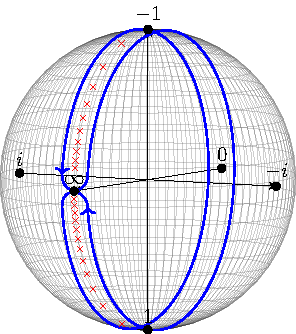
\includegraphics{thermal_field_theory/plots/integral_cont.pdf}        
    \end{subfigure}
    \begin{subfigure}{0.18\textwidth}
        \centering
        \begin{tikzpicture}
            \draw[-stealth] (0, 0) -- (1, 0);
        \end{tikzpicture}
        \end{subfigure}
    \begin{subfigure}{0.4\textwidth}
        \centering
        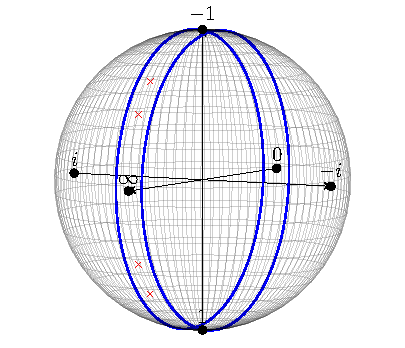
\includegraphics{thermal_field_theory/plots/integral_cont2.pdf}
    \end{subfigure} 
    \caption{The integral contour $\gamma$, and the result of deforming it into to contours close to the real line.
    The red crosses illustrate the poles of $n_B$.}
    \label{fig:integral contours}
\end{figure}
In the last line, we have changed variables $z \rightarrow -z$ in the first integral, and exploited the property $n_B(-i z) = -1 - n_B(iz)$.
As $n_B(iz)$ is analytic on the real line, the result is the sum of residues of $f$ in the lower half plane.
The function
\begin{equation}
    f(z) = \frac{1}{(z + i \mu)^2 + \omega^2} 
    = \frac{i}{2 \omega } 
    \left(
        \frac{1}{z + i(\mu + \omega)} - \frac{1}{z + i(\mu - \omega)}
    \right)
\end{equation}
obeys the assumed properties, as it has poles at
$z = - i (\mu \pm \omega)$, with residue $1 / 2 \omega$, so the function defined in \autoref{i func} may be written \footnote{Assuming $\omega>\mu$.}
\begin{equation}
    i(\omega, \mu) 
    % = \left(\frac{-2 \pi i^2}{2 \pi \omega}\right)
    % [1 + n_B(\omega + \mu) + n_B(\omega - \mu)].
    = \frac{1}{2\omega}
    [1 + n_B(\omega + \mu) + n_B(\omega - \mu)].
\end{equation}

Using the anti-derivative of the Bose distribution, we get the final form of \autoref{j func}
\begin{equation}
    j(\omega, \mu) = \int \dd \omega'\, \omega' i(\omega', \mu)
    =  
    \frac{1}{2}\omega + \frac{1}{2\beta} 
    \left[
        \ln\left(1 - e^{-\beta(\omega - \mu)}\right)
        + \ln\left(1 - e^{-\beta(\omega + \mu)}\right)
    \right]
    + g'(\beta).
\end{equation}
The extra $\omega$-independent term $g'(\beta)$ is an integration constant.
We see there are temperature dependent terms, one due to the particle and one due to the anti-particle, and one due to the antiparticle, as they have opposite chemical potentials.


% Inkludere Figur, og den fermionske versjonen
% \documentclass[tikz]{standalone}

\usepackage{tikz}
\usepackage{pgfplots}
\pgfplotsset{compat=1.9}

\usetikzlibrary{math}
\usetikzlibrary{arrows.meta}


\begin{document}
\begin{tikzpicture}
    \tikzmath{
        \r = 0.1;   % radius of curve to inf
        \t = 6;     % how far the curve is rotaed
    }
    \begin{axis}[axis lines=center, ticks=none, view/h=120, view/v=5]
    % Sphere
    \addplot3[%
    opacity = 0.1,
    mesh,
    black,
    z buffer = sort,
    samples = 50,
    variable = \u,
    variable y = \v,
    domain = 0:180,
    y domain = 0:360,
    ]
    ({cos(u)*sin(v)}, {sin(u)*sin(v)}, {cos(v)});
    % Large circles
    \addplot3[%
        domain=rad(\t):2*pi-rad(\t),
        samples=100,
        samples y=0,
        no marks,
        smooth,
        thick,
        blue,
        ->
    ]
    (
        {sqrt(1 - \r^2)*cos(deg(x))}, 
        {\r}, 
        {sqrt(1 - \r^2)*sin(deg(x))}
    );
    %
    \addplot3[%
        domain=rad(\t):2*pi-rad(\t),
        samples=100,
        samples y=0,
        no marks,
        smooth,
        thick,
        blue,
        <-
    ]
    (
        {sqrt(1 - \r^2)*cos(deg(x))}, 
        {-\r},
        {sqrt(1 - \r^2)*sin(deg(x))}
    );
    % Small curves touching infinity
    \addplot3[%
        domain=pi:2*pi,
        samples=10,
        samples y=0,
        no marks,
        smooth,
        thick,
        blue
    ]
    (   {1*cos(\t) - \r*sin(deg(x))*sin(\t)},
        {\r*cos(deg(x))+0.004},
        {1*sin(\t) + \r*sin(deg(x))*cos(\t)}
    );
    %
    \addplot3[%
        domain=0:pi,
        samples=10,
        samples y=0,
        no marks,
        smooth,
        thick,
        blue
    ]
    (   {1*cos(-\t) - \r*sin(deg(x))*sin(-\t)},
        {\r*cos(deg(x))+0.004},
        {1*sin(-\t) + \r*sin(deg(x))*cos(-\t)}
    );
    % Points
    \addplot3[
        mark=*,
        black, 
        point meta=explicit symbolic,
        nodes near coords
        ]
    coordinates {(1,0,0)[$\infty$]};
    \addplot3[
        mark=*,
        black, 
        point meta=explicit symbolic,
        nodes near coords
        ]
    coordinates {(-1,0,0)[$0$]};
    \addplot3[
        mark=*,
        black, 
        point meta=explicit symbolic,
        nodes near coords
        ]
    coordinates {(0,0,1)[$-1$]};
    \addplot3[
        mark=*,
        black, 
        point meta=explicit symbolic,
        nodes near coords
        ]
    coordinates {(0,0,-1)[$1$]};
    \addplot3[
        mark=*,
        black, 
        point meta=explicit symbolic,
        nodes near coords
        ]
    coordinates {(0,1,0)[$-i$]};
    \addplot3[
        mark=*,
        black, 
        point meta=explicit symbolic,
        nodes near coords
        ]
    coordinates {(0,-1,0)[$i$]};
    \addplot3[
        domain=2:15,
        samples=10,
        red,
        only marks,
        mark=x,
        ]
    (
        {cos(deg( pi/2* (ln(20) - ln(x))/ln(20)) )},
        {0},
        {sin(deg( pi/2* (ln(20) - ln(x))/ln(20)) ))}
    );
    \addplot3[
        domain=2:18,
        samples=12,
        red,
        only marks,
        mark=x,
        ]
    (
        {cos(deg( -pi/2* (ln(20) - ln(x))/ln(20)) )},
        {0},
        {sin(deg( -pi/2* (ln(20) - ln(x))/ln(20)) ))}
    );
    \end{axis}
\end{tikzpicture}
\end{document}

\section{Interacting scalar}
\label{section:interacting scalar}

We now study a scalar field with a $\lambda \varphi^4$ interaction term.
We write the Lagrangian in the form
\begin{equation*}
    \Ell = \Ell^{(0)} + \Ell^{(I)}, \quad 
    \Ell^{(0)} = 
    \frac{1}{2} \partial_\mu \varphi \partial^\mu \varphi - m^2 \varphi^2 , \quad
    \Ell^{(I)} = - \frac{\lambda}{4!} \varphi^4
\end{equation*}
$\Ell^{(I)}$ is called the interaction term, and makes it impossible to exactly solve for the partition function.
Instead, we turn to perturbation theory.
The canonical partition function in this theory is
\begin{equation}
    Z = \Tr{e^{- \beta \hat H}}
    = \int_S \D \varphi \, \exp{
        - \int_\Omega \dd X \left(\Ell_E^{(0)} + \Ell_E^{(I)}\right)
    }
    = \int_S \D \varphi \, e^{-S_0} e^{-S_I}.
\end{equation}
Here, $S_0$ and $S_I$ denote the Euclidean action due to the free and interacting Lagrangian, respectively.
The domain of integration $S$ is again periodic field configurations $\varphi(\beta, \vec x) = \varphi(0, \vec x)$.
We may write the free energy as
\begin{equation*}
    - \beta F = \ln
    \left[
        \int_S \D \varphi \, e^{-S_0} \sum_n \frac{1}{n!} {(-S_I)}^n
    \right]
    = \ln Z_0 
    + \ln Z_I ,
\end{equation*}
where $Z_0$ is the partition function of the free theory.
The correction to the partition function is thus given by
\begin{equation}
    Z_I = \sum_{n=0}^\infty \frac{(-1)^n}{n!} \ex{{S_I}^n}_0,
\end{equation}
where
\begin{equation}
    \ex{A}_0 = \frac{
        \int_S \D \varphi \, A \, e^{-S_0} }
    {\int_S \D \varphi \, e^{-S_0}}.
\end{equation}

To evaluate expectation values of the form $\ex{\varphi(X_1) ... }_0$, we introduce the partition function with a source term
\begin{align}
    Z[J] = \int_S \D \varphi \, \exp{
        - \frac{1}{2} \int_\Omega \dd X \, \varphi (-\partial_E^2 + m^2) \varphi
        + \int_\Omega \dd X \, J \varphi
    }.
\end{align}

Thermal propagators are the generalization of the time-ordered two-point functions $\ex{T\{\varphi(x) \varphi(y) \}}$ of the vacuum formalism.
For some differential operator $D^{-1}$, the thermal propagator is defined as
\begin{equation}
    D^{-1} D(X, Y) = \beta \delta(X - Y).
\end{equation}
The Fourier transformed propagator is, assuming $D(X, Y) = D(X-Y, 0)$,
\begin{align}
    \nonumber
    \tilde D(K, K') 
    & = \frac{1}{V \beta^3} \int_{\Omega} \dd X \dd Y \, 
    D(X, Y) \exp(- i [X\cdot K + Y\cdot K']) \\ \nonumber
    & = \frac{1}{V \beta^3} \int_{\Omega} \dd X' \dd Y' \, D(X', 0) 
    \exp(- i [X'\cdot \frac{1}{2} (K - K') + Y\cdot (K + K')]) \\
    & = \frac{1}{V \beta^2} \tilde D(K) \delta(K + K'),
\end{align}
where
\begin{equation}
    \tilde D(K) = \int \dd X e^{iK\cdot X} D(X, 0).
\end{equation}
We write the thermal propagator of the free field as $D_0(X, Y)$.
With this, we may complete the square,
\begin{align}
    Z[J] = Z[0]\exp{\frac{1}{2} \int_{\Omega} \dd X \dd Y J(X) D_0(X, Y) J(Y)}
    = Z[0] \exp(W[J])
\end{align}
We can now write
\begin{equation}
    \ex{\varphi(X)\varphi(Y)}_0 
    = \frac{1}{Z[0]}
    \frac{\delta}{\delta J(X)} \frac{\delta}{\delta J(Y)} 
    Z[J] \Big|_{J=0} 
    = D_0(X, Y).
\end{equation}
This generalizes to higher order expectation values,
\begin{equation}
    \ex{\varphi(X_i) \dots \varphi(X_n)}_0
    = \frac{1}{Z[0hju]} \left(\prod_{i=1}^n \frac{\delta}{\delta J(X_i)}\right) 
    Z[J] \Big|_{J=0},
\end{equation}

Using Wick's theorem, as described in \autoref{section:path integral}, the expectation values we are evaluating can be written
\begin{align*}
    \ex{{S_I}^m}_0 & 
    = \left(- \frac{\lambda }{4!}\right)^m 
    \int_{\Omega} \dd X_1 \dots \dd X_m
    \ex{\varphi^4(X_1) \dots \varphi^4(X_m)}_0 \\ 
    & \quad
    = \left(- \frac{\lambda }{4!}\right)^m 
    \int_{\Omega} \dd X_1 \dots \dd X_m \sum_{\{a, b\}}
    \ex{\varphi(X_{a(1)}) \varphi(X_{b(1)})}_0
    \dots
    \ex{\varphi(X_{a(2m)}) \varphi(X_{b(2m)})}_0
\end{align*}
where $X_i$ for $i>m$ is defined to equal $X_j$, where $j = i \mod m$.
More simpliy,  $X_{m + i} = X_i$.
The functions $a,\,b$ represents a possible pairing, as described in \autoref{section:path integral}.
Inserting the Fourier expansions of the field gives
\begin{align*}
    & \ex{{S_I}^m}_0 \\
    &\quad 
    = \left(-\frac{\lambda }{4!}\right)^m 
    \int_{\Omega} \dd X_1 \dots \dd X_m
    (V \beta)^2 \int_{\tilde \Omega} \dd K_1 ... \dd K_{2m} \sum_{\{a, b\}} \\
    & \quad \quad \quad \quad\quad \quad \quad
    \ex{\varphi(K_{a(1)}) \varphi(K_{b(1)})}_0
    \dots
    \ex{\varphi(K_{a(2m)}) \varphi(K_{b(2m)})}_0     
    \exp(i {\sum}_{i=1}^{m} X_i \cdot K_i)\\ 
    & \quad  
    = \left(-\frac{\lambda }{4!}\right)^m 
    \frac{(V \beta)^{2m} \beta^m}{(V \beta^2)^{2m}}
    \int_{\tilde \Omega} \dd K_1 ... \dd K_{2m} \sum_{\{a, b\}} \\
    & \quad \quad \quad \quad \quad \quad \quad \quad \quad
    \tilde D(K_{a(1)}) \delta(K_{a(1)} + K_{b(1)}) \dots 
    \tilde D(K_{a(2m)}) \delta(K_{a(2m)} + K_{b(2m)})
    \prod_{i=1}^m \delta\left(X_i \cdot {\sum}_{j=0}^3 K_{i + jm}\right) \\
    & \quad 
    = \left(-\frac{\lambda \beta}{4!}\right)^m 
    \prod_{i=1}^{2m} \int_{\tilde \Omega} 
    \left( \dd K_i \frac{1}{\beta} \tilde D(K_i)  \right) 
    \prod_{i=1}^m \delta\left(X_i \cdot {\sum}_{j=0}^3 K_{i + jm}\right)
    \sum_{\{a, b\}} 
    \prod_{n=1}^{2m}\delta(K_{a(k)} + K_{b(k)}).
\end{align*}
Here we have used that $V \beta^2 \tilde D_0(K, P) = \tilde D_0(K) \delta(P + K)$, where $\tilde D_0(K)$ is the thermal propagator for the free field.
In this case, it is
\begin{equation}
    \tilde D_0(K) = \tilde D_0(\omega_n, \vec k) = \frac{1}{\omega_k^2 + \omega_n^2}.
\end{equation}
This expectation value can be represented graphically using Feynman diagrams.
The thermal $\lambda \varphi^2$-theory gets the prescription

\begin{align}
    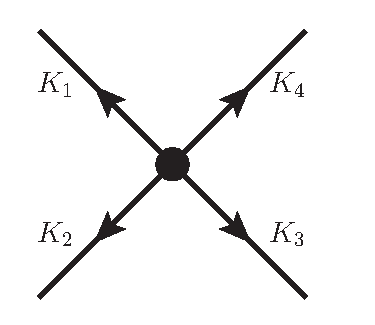
\includegraphics[width=0.15\textwidth, valign=c]{figurer/feynman-diagram/phi-4_vertex.eps}
    & = -\lambda \beta
    \delta \left({\sum}_i K_i \right), \\ \nonumber \\
    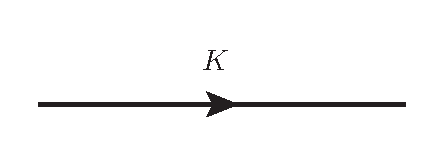
\includegraphics[width=0.2\textwidth, valign=c]{figurer/feynman-diagram/phi-4_propagator.eps}
    & = \frac{1}{\beta} D_0(K).
\end{align}
Lastly, one has to integrate over internal momenta and divide by the symmetry factor of the diagram $s$, which is described in detail in~\cite{Peskin:IntroQFT}.

Calculating $\ex{{S_I}^n}_0$ boils down to the sum of all possible Feynman diagrams with $n$ vertices.
The first example is 
\begin{align}
    \ex{S_I}_0 =
    \frac{1}{8} 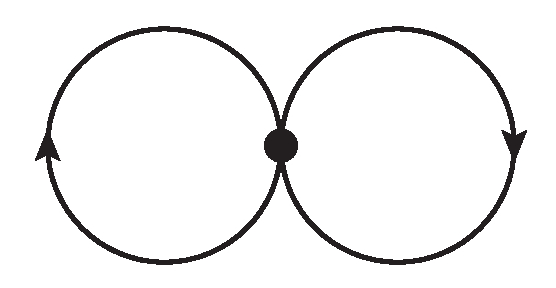
\includegraphics[width=0.15\textwidth, valign=c]{figurer/feynman-diagram/phi-4_loop_notext.eps}.
\end{align}

In \autoref{section:path integral}, we saw that the sum of all vacuum diagrams is the exponential of the sum of all \emph{connected} diagrams, so the free energy of the interacting theory is given by
\begin{equation}
    - \beta F = \ln Z_0 + \Sigma(\mathrm{all\,\, connected\,\, diagrams}).
\end{equation}

\section{Fermions}

The phase factor $e^{i\theta}$ that was introduced in \autoref{section:imaginary-time formalism} can be determined by studying the properties of the thermal Greens function.
The thermal Greens function may be written 
\begin{equation*}
    D(X_1, X_2) = D(\vec x, \vec y, \tau_1, \tau_2) 
    = \ex{e^{-\beta \hat H} \T{ \hat \varphi(X_1) \hat \varphi(X_2) } }.
\end{equation*}
$\T{...}$ is time-ordering operator,
% the temperature ordering operator, analogous to the time ordering operator from scattering theory.
and is defined as
\begin{equation*}
    \T{\varphi(\tau_1)\varphi(\tau_2)}
    = \theta(\tau_1 - \tau_2) \varphi(\tau_1)\varphi(\tau_2)
    + \nu \theta(\tau_2 - \tau_1) \varphi(\tau_2)\varphi(\tau_1),
\end{equation*}
where $\nu = \pm 1$ for bosons and fermions respectively, and $\theta(\tau)$ is the Heaviside step function.
In the same way that $i \hat H$ generates the time translation of a quantum field operator through $\hat\varphi(x) = \hat\varphi(t, \vec x) = e^{it\hat H} \hat \varphi(0, \vec x) e^{-it\hat H} $, the imaginary-time formalism implies the relation
\begin{equation}
    \hat\varphi(X) = \hat\varphi(\tau, \vec x) 
    = e^{\tau\hat H} \hat \varphi(0, \vec x) e^{-\tau \hat H}.
\end{equation}
Using $\one = e^{\tau \hat H} e^{-\tau \hat H}$ and the cyclic property of the trace, we show that, assuming $\beta>\tau>0$,
\begin{align*}
    G(\vec x, \vec y, \tau, 0)
    & = \ex{e^{-\beta \hat H} \T{\varphi(\tau, \vec x) \varphi(0, \vec y)}} \\
    & = \frac{1}{Z} \Tr{
        e^{-\beta \hat H} \varphi(\tau, \vec x) \varphi(0, \vec y)
    } \\
    & = \frac{1}{Z} \Tr{
        \varphi(0, \vec y) e^{-\beta \hat H} \varphi(\tau, \vec x)
    } \\
    & = \frac{1}{Z} \Tr{
        e^{-\beta \hat H} e^{\beta \hat H} \varphi(0, \vec y) 
        e^{-\beta \hat H} \varphi(\tau, \vec x)
    } \\
    & = \frac{1}{Z} \Tr{
        e^{-\beta \hat H} \varphi(\vec y, \beta) \varphi(\tau, \vec x)
    } \\
    & = \nu \ex{
        e^{-\beta \hat H} \T{ \varphi(\tau, \vec x) \varphi( \beta, \vec y) }
    }.
\end{align*}
This implies that $\varphi(0, x) = \nu \varphi(\beta, \varphi)$, which shows that bosons are periodic in time, as stated earlier, while fermions are anti-periodic.

The Lagrangian density of a free fermion is
\begin{equation}
    \Ell = \bar \psi \left( i \slashed{\partial} - m \right) \psi.
\end{equation}
This Lagrangian is invariant under the transformation $\psi \rightarrow e^{-i \alpha} \psi$, which by Nöther's theorem results in a conserved current
\begin{equation}
    j^\mu = \pdv{\Ell}{(\partial_\mu \psi)} \delta \psi=  \bar \psi \gamma^\mu \psi.
\end{equation}
The corresponding conserved charge is 
\begin{equation}
    Q = \int_V \dd^3 x\, j^0 = \int_V \dd^3 x \, \bar \psi \gamma^0 \psi.
\end{equation}
We can now use our earlier result for the thermal partition function, \autoref{Thermal partition function}, only with the substitution $\He \rightarrow \He - \mu \bar \psi \gamma^0 \psi$, and integrate over anti-periodic $\psi$'s:
\begin{equation*}
    Z = \Tr{e^{-\beta(\hat H - \mu \hat Q)}}
    = \prod_{a b}\int \D \psi_a\D \pi_b \exp{
        \int_{\Omega} \dd X \, 
        \left(
            i\dot \psi \pi - \He(\psi, \pi) + \mu \bar \psi \gamma^0 \psi
        \right)
    },
\end{equation*}
where $a, b$ are the spinor indices.
The canonical momentum corresponding to $\psi$ is
\begin{equation}
    \pi = \pdv{\Ell}{(\partial_0 \psi)} = i \bar \psi \gamma^0,
\end{equation}
and the Hamiltonian density is 
\begin{equation}
    \He = \pi \dot\psi - \Ell
    = \bar \psi (-i\gamma^i\partial_i + m) \psi
\end{equation}
which gives
\begin{equation}
    \Ell_E = 
    - i \pi \dot\psi + \He(\psi, \pi) - \mu \bar \psi \gamma^0 \psi
    = \bar\psi[\gamma^0 (\partial_\tau - \mu) - i\gamma^i \partial_i + m] \psi,
\end{equation}
By using the Grassman-version of the Gaussian integral formula, the partition function can be written
\begin{align*}
    Z & = \prod_{a b}\int \D \psi_a\D \bar \psi_b 
    \exp{
        - \int_\Omega \dd X \, \bar \psi
        \left[
            \tilde\gamma_0(\partial_\tau -\mu) -  i \gamma^i \partial_i + m
        \right]
        \psi
    }\\
    & = C \prod_{a b}\int \D \tilde \psi_a\D \tilde {\bar \psi}_b 
    \exp{
        - \int_{\tilde \Omega} \dd K \, \tilde {\bar \psi}
        \left[
            i \tilde\gamma_0(\omega_n + i\mu) + i \gamma_i p_i + m
        \right]
        \tilde \psi
    } \\
    & = C \prod_{a b}\int \D \tilde \psi_a\D \tilde {\bar \psi}_b 
    e^{- \langle \tilde {\bar \psi}, D_0^{-1} \psi\rangle} 
    = \det(D_0^{-1}).
\end{align*}
In the second line, we have inserted the Fourier expansion of the field, as defined in \autoref{Conventions and notation}, and changed variable of integration, as we did for the scalar field.
The linear operator in this case is 
\begin{equation}
    D_0^{-1} = i \gamma^0 (-i\partial_\tau + i\mu) - (- i \gamma^i) \partial_i + m
    = 
    \beta [i \tilde \gamma_a p_a + m ].
\end{equation}
This equality must be understood as an equality between linear operators, which are represented in different bases.
We introduced the notation $p_{n;a} = (\omega_n + i \mu, p_i)$ and use the Euclidean gamma matrices, as defined in \autoref{Conventions and notation}.
We use the fact that 
\begin{equation*}
    \det(i\tilde\gamma_a p_a + m)
    = \det(\gamma^5 \gamma^5)
    \det(i\tilde\gamma_a p_a + m)
    = \det[\gamma^5 (i\tilde\gamma_a p_a + m) \gamma^5]
    = \det(-i\tilde\gamma_a p_a + m),
\end{equation*}
Let $\tilde D = -i\tilde\gamma_a p_a + m$, which means we can write
\begin{equation}
    Z = \sqrt{\det(D)\det(\tilde D)} = \sqrt{\det(D\tilde D)} = \det[\one(p_a p_a + m^2)]^{1/2},
\end{equation}
where we have used the anti-commutation rule for the Euclidean gamma-matrices, $\acom{\gamma_a}{\gamma_b} = 2 \delta_{ab}$.
It is important to keep in mind that the determinant here refers to linear operators on the space of spinor functions.
\begin{align}
    \nonumber
    \ln(Z) & = \ln\left\{\det[\one(p_a p_a + m^2)]^{1/2}\right\}
    = \frac{1}{2} \Tr{\ln[\one(p_a p_a + m^2)]} \\
    & = \frac{1}{2} \int_{\tilde \Omega} \dd K \ln[\one \beta^2 (p_a p_a + m^2)]_{aa}
\end{align}
As the matrix within the logarithm is diagonal, the matrix-part of the trace is trivial, and the free energy may be written
\begin{equation}
    \beta \Ef
    = - 2 \int_{\tilde \Omega} \dd X \,  \ln\{ \beta^2[(\omega_n + i\mu)^2 + \omega_k^2]\} .
\end{equation}
Using the fermionic version of the thermal sum from \autoref{section:thermal sum} gives the answer
\begin{equation}
    \Ef = 2 \int\frac{\dd^3 p}{(2\pi)^3} \, 
    \left[
        \beta \omega_k
        + \frac{1}{\beta} \ln\left(1 + e^{-\beta(\omega_k-\mu)}\right)
        + \frac{1}{\beta} \ln\left(1 + e^{-\beta(\omega_k+\mu)}\right)
    \right].
\end{equation}
We see again that the temperature-independent part of the integral diverges, and must be regulated.
There are two temperature-dependent terms, one from the particle and one from the anti-particle.

% Ha bedre overgang til fermionic path integral
% Regne ut trace spinor-indekser bedre

\bibliographystyle{unsrt}
\bibliography{referanser}


\clearpage
\begin{appendices}
    Throughout this text, \emph{natural units} are used.
These units are defined so that
\begin{equation}
    \hbar = c = k_B = 1,
\end{equation}
where $\hbar$ is the Planck reduced constant, $k_B$ is the Boltzmann constant, and $c$ is the speed of light.
These constants will therefore be dropped from all expressions.
They can be reintroduced using dimensional analysis.
In natural units, \emph{mass dimension} is the only engineering dimension.
Dimensionfull results are given in units of electronvolt (eV), or pion-masses, 
\begin{equation}
    m_\pi = 131 \, \text{MeV}.
\end{equation}

The Minkowski metric convention used is the ``mostly minus'',
\begin{equation}
    g_{\mu \nu} = \mathrm{diag}(1, -1, -1, -1).
\end{equation}
The Fourier transform used in this text is defined by
\begin{align*}
    \F{f(x)}(p) = \tilde f(p) = \int \dd x\, e^{i p x}f(x), \quad 
    \FInv{\tilde f(p)}(x) = f(x) = \int \frac{\dd p}{2 \pi}\, e^{- i p x} \tilde f(p).
\end{align*}
We employ the \emph{Einstiein summation convention}, in which pairwise matching indices are summed.
That is,
\begin{equation}
    a_i b_i = \sum_i a_i b_i = a_1 b_1 + \dots.
\end{equation}
For Minkowski-space indices, $\mu$, $\nu$, $\rho$ and $\sigma$, the metric raises and lower indices, and summation should always be over one raised and one lowered index,
\begin{equation}
    a_\mu b^\mu = g_{\mu\nu} a^\mu b^\nu 
    = a^0 b^0 - a^1 b^1 - \dots.
\end{equation}

    \section{Covariant derivative}

In \chpt at finite isospin chemical potential $\mu_I$, the covariant derivative acts on functions $A(x): \Em_4 \rightarrow \lieg{SU}{2}$, where $\Em_4$ is the space-time manifold. It is defined as 
\begin{equation}
    \nabla_\mu A(x) = \partial_\mu A(x) - i \com{v_\mu}{A(x)}, 
    \quad v_\mu = \frac{1}{2} \mu_I \delta_\mu^0 \tau_3.
\end{equation}
The covariant derivative obeys the product rule, as
\begin{equation*}
    \nabla_\mu (A B) 
    = (\partial_\mu A) B + A (\partial_\mu B) - i \com{v_\mu}{AB}
    = (\partial_\mu A - i \com{v_\mu}{A})B + A(\partial_\mu B- i \com{v_\mu}{B}) 
    = (\nabla_\mu A)B + A (\nabla_\mu B).
\end{equation*}
Decomposing a 2-by-2 matrix $M$, as described in \autoref{section:algebra bases}, shows that the trace of the commutator of $\tau_b$ and $M$ is zero:
\begin{equation*}
    \Tr{\com{\tau_a}{M}]} = M_b\Tr{ \com{\tau_a}{\tau_b}} = 0.
\end{equation*}
Together with the fact that $\Tr{\partial_\mu A} = \partial_\mu \Tr{A}$, this gives the product rule for invariant traces:
\begin{equation*}
    \Tr{A \nabla_\mu B} = \partial_\mu \Tr{AB} - \Tr{(\nabla_\mu A) B}.
\end{equation*}
This allows for the use of the divergence theorem when doing partial integration.
Let $\Tr{K^\mu}$ be a space-time vector, and $\Tr{A}$ scalar. 
Let $\Omega$ be the domain of integration, with coordinates $x$ and $\partial \Omega$ its boundary, with coordinates $y$. Then, 
\begin{align*}
    \int_\Omega \dd x \, \Tr{A \nabla_\mu K^\mu} = \int_{\partial\Omega} \dd y\, n_\mu \Tr{A K^\mu} - \int_\Omega \dd x \, \Tr{(\nabla_\mu A) K^\mu},
\end{align*}
where $n_\mu$ is the normal vector of $\partial \Omega$~\cite{Carroll:space-time}.
This makes it possible to do partial integration and discard surface terms in the \chpt Lagrangian, given the assumption of no variation on the boundary.

    \section{Integrals}
\subsection{Gaussian integrals}
A useful integral is the Gaussian integral,
\begin{equation}
    \int_\R \dd x \, \exp(- \frac{1}{2} a x^2) = \sqrt{\frac{2 \pi}{a}},
\end{equation}
for $a \in \R$. The imaginary version,
\begin{equation}
    \int_R \dd x \, \exp(i \frac{1}{2} a x^2 ) 
\end{equation}
does not converge. However, if we change the contour of integration slightly, by rotating it clockwise to $C = \R(1 + i\epsilon)$,
\begin{figure}
    \begin{subfigure}{0.4\textwidth}
        \begin{tikzpicture}
            \draw (-2, 0) -- (2, 0) node[right] {$\mathrm{Re}(x)$};
            \draw (0, -2) -- (0, 2) node[above] {$\mathrm{Im}(x)$};
            \draw[->, thick] (-1.8, 0) -- (1.8, 0);
        \end{tikzpicture}    
    \end{subfigure}
    \begin{subfigure}{0.18\textwidth}
        \begin{tikzpicture}
            \draw[->] (-1, 0) -- (1, 0);
        \end{tikzpicture}
    \end{subfigure}
    \begin{subfigure}{0.4\textwidth}
        \begin{tikzpicture}
            \draw (-2, 0) -- (2, 0) node[right] {$\mathrm{Re}(x)$};
            \draw (0, -2) -- (0, 2) node[above] {$\mathrm{Im}(x)$};
            \draw[->, thick] (-1.8, -0.1) -- (1.8, 0.1);
        \end{tikzpicture}    
    \end{subfigure}
\end{figure}

    \chapter{Functional derivatives}
\label{section:Functional derivative}

Functional derivatives generalize the notion of gradients and directional derivatives.
A function $f(x)$ has a gradient
\begin{equation}
    \dd f_{x_0} = \pdv{f}{x_i} \Big|_{x_0} \dd x_i.
\end{equation}
The derivative in a particular direction $v = v^i \partial_i$ is 
\begin{equation}
    \dv{\epsilon} f(x_i + \epsilon v_i) \Big|_{\epsilon = 0} 
    = f(x) + \dd f_x (v) = f(x) + \pdv{f}{x^i}v_i.
\end{equation}
This is generalized to functionals through the definition of the functional derivative and the variation of a functional.
Let $F[f]$ be a functional, i.e., a machine that takes in a function and returns a number or a function.
The obvious example in our case is the action, which takes in one or more field configurations, and returns a single real number.
We will assume here that the functions have the domain $\Omega$, with coordinates $x$.
The functional derivative is defined as
\begin{equation}
    \delta F[f]
    =
    \dv{\epsilon} F[f + \epsilon \eta] \Big|_{\epsilon = 0}
    = \int_\Omega \dd x \, \frac{\delta F[f]}{\delta f(x)} \eta(x).
\end{equation}
$\eta(x)$ is here an arbitrary function, but we will make the assumption that it as well as all its derivatives are zero at the boundary of its domain $\Omega$, i.e., $\eta(\partial \Omega) = 0$.
This allows us to discard surface terms stemming from partial integration, which we will use frequently.
We may use the definition to derive one of the fundamental relations of functional derivation.
Take the functional $F[f] = f(x)$. 
Then,
\begin{equation}
    \label{Functional derivative delta identity}
    \delta F[f] = \dv{\epsilon} [f(x) + \epsilon \eta(x)] \Big|_{\epsilon = 0}
    = \eta(x) = \int \dd y \, \delta(x - y) \eta(y)
\end{equation}
This leads to the identity
\begin{equation}
    \frac{\delta f(x)}{\delta f(y)} = \delta(x - y),
\end{equation}
for any function $f$.
Higher functional derivatives are defined similarly, by applying functional variation repeatedly
\begin{equation}
    \delta^n F[f] = \dv{\epsilon} \delta^{n-1}F[f + \epsilon \eta_n] \big|_{\epsilon=0}
    = \int \left(\prod_{i=1}^n \dd x_i\right)
    \frac{\delta^n F[f]}{ \delta f(x_n)\dots\delta f(x_1)} \left(\prod_{i=1}^n \eta_i(x_i)\right).
\end{equation}
If we can write the functional $F[f]$ in terms of a new variable, $g(y)$, then the chain rule for functional derivatives is
\begin{equation}
    \fdiff{F[f]}{f(x)} = \int \dd y \, \fdiff{F[f]}{g(y)} \fdiff{g(y)}{f(x)}.
\end{equation}

A functional may be expanded in a generalization of the Taylor series, 
\begin{equation}
    F[f_0 + f] = F[f_0] + \int_\Omega \dd x \, f(x) \frac{\delta F[f_0]}{\delta f(x)}
    + \frac{1}{2!}\int_\Omega \dd x \dd y \, f(x) f(y) \frac{\delta^2 F [f_0]}{\delta f(x) \delta f(y)}
    + \dots
\end{equation}
Her, the notation
\begin{equation}
    \fdiff{F[f_0]}{f(x)}
\end{equation}
indicate that the functional $F[f]$ is first differentiated with respect to $f$, the evaluated at $f = f_0$.
As an example, the Klein-Gorodn action
\begin{equation}
    S[\varphi] = - \frac{1}{2}\int_\Omega \dd x \, \varphi(x) (\partial^2 + m^2) \varphi(x).
\end{equation}
Using \autoref{Functional derivative delta identity} and partial integration,
\begin{align}
    \nonumber
    \funcdv{\varphi(x)} S[\varphi] 
    & = 
    - \frac{1}{2} \int_\Omega \dd y \, 
    [\delta(x - y)(\partial_y^2 + m^2)\varphi(y) + \varphi(y) (\partial_y^2 + m^2)\delta(x - y)] \\
    & = 
    - \int_\Omega \dd y \, 
    \delta(x - y)(\partial_y^2 + m^2)\varphi(y) 
    = (\partial_x^2 + m^2)\varphi(x)
\end{align}
The second derivative is
\begin{equation}
    \frac{\delta^2S[\varphi]}{\delta \varphi(x)\delta \varphi(y)}
    =
    \funcdv{\varphi(x)} (\partial_y^2 + m^2)\varphi(y)
    = 
    (\partial_y^2 + m^2) \delta(x - y).
\end{equation}


\subsection*{Gaussian integrals}
\label{section:gaussian integrals}

\begin{figure}[ht]
    \centering
    \begin{tikzpicture}
        \draw (-2, 0) -- (2, 0) node[right] {$\mathrm{Re}(x)$};
        \draw (0, -2) -- (0, 2) node[above] {$\mathrm{Im}(x)$};
        \draw[->, thick] (-1.75, 0.1) -- (1.8, 0.1);
        \draw[->, thick] (1.8, 0.15) arc (10:45:1.8);
        \draw[->, thick] ({1.8/sqrt(2)}, {1.8/sqrt(2)}) -- ({-1.8/sqrt(2)}, {-1.8/sqrt(2)});
        \draw[->, thick] ({-1.8/sqrt(2)}, {-1.8/sqrt(2)}) arc (225:180:1.8);
    \end{tikzpicture}
    \caption{Wick rotation}
    \label{Wick rotation}
\end{figure}


A useful integral is the Gaussian integral,
\begin{equation}
    \int_\R \dd x \, \exp(- \frac{1}{2} a x^2) = \sqrt{\frac{2 \pi}{a}},
\end{equation}
for $a \in \R$. The imaginary version,
\begin{equation}
    \int_R \dd x \, \exp(i \frac{1}{2} a x^2 )
\end{equation}
does not converge. However, if we change $a \rightarrow a + i\epsilon$, the integrand is exponentially suppressed.
\begin{equation}
    f(x) = \exp(i \frac{1}{2}a x^2) \rightarrow
    \exp(i\frac{1}{2}a x^2 - \frac{1}{2} \epsilon  x^2).
\end{equation}
As the integrand falls exponentially for $x\rightarrow \infty$ and contains no poles in the upper right nor lower left quarter of the complex plane, we may perform a wick rotation by closing the contour as shown in \autoref{Wick rotation}.
This gives the result
\begin{equation}
    \label{complex gauss 1D}
    \int_\R \dd x \, \exp(i \frac{1}{2}(a + i\epsilon) x^2) 
    = \int_{\sqrt{i}\R} \dd x \, \exp(i\frac{1}{2} ax^2)
    = \sqrt{i} \int_\R \dd y\, \exp(-\frac{1}{2} (-a) y^2) = \sqrt{\frac{2 \pi i}{(-a)}}
\end{equation}
where we have made the change of variable $y = (1+i)/\sqrt{2} x = \sqrt{i} x$.
In $n$ dimensions, the Gaussian integral formula generalizes to
\begin{equation}
    \int_{\R^n} \dd^n x \, \exp{-\frac{1}{2} x_n A_{nm} x_m } =\sqrt{\frac{(2 \pi)^n}{\det(A)}},
\end{equation}
where $A$ is a matrix with $n$ real, positive eigenvalues.
We may also generalize \autoref{complex gauss 1D},
\begin{align}
    \int_{\R^n} \dd^n x \, \exp{i\frac{1}{2} x_n( A_{nm} + i \epsilon \delta_{nm}) x_m } =\sqrt{\frac{(2 \pi i )^n}{\det(-A)}}.
\end{align}
The final generalization is to functional integrals,
\begin{align}
    \int \D \varphi \, \exp(- \frac{1}{2} \int \dd x \, \varphi(x) A \varphi(x) )
    = C (\det(A))^{-1/2},
    \int \D \varphi \, \exp(i\frac{1}{2} \int \dd x \, \varphi(x) A \varphi(x) )
    = C (\det(-A))^{-1/2}.
\end{align}
$C$ is here a divergent constant, but will either fall away as we are only looking at the logarithm of $I_\infty$ and are able to throw away additive constants, or ratios between quantities which are both multiplied by $C$.

The Gaussian integral can be used for the stationary phase approximation.
In one dimension, it is
\begin{equation}
    \int \dd x \, \exp{i \alpha f(x)} 
    \approx \sqrt{\frac{2 \pi }{f''(x_0)}}\exp{ f(x_0)}, 
    \, \alpha\rightarrow \infty,
\end{equation}
where the point $x_0$ is defined by $ f'(x_0) = 0$. 
The functional generalization of this is
\begin{equation}
    \int \D \varphi \exp{i S[\varphi]}
    \approx 
    C \det(- \frac{\delta^2 S[\varphi_0]}{\delta \varphi^2})
    \exp{i \alpha S[\varphi_0]  },
\end{equation}
Here, $S[\varphi]$ is a general functional of $\varphi$, we have used the Taylor expansion, and $\varphi_0$ obeys
\begin{equation}
    \funcdv{\varphi(x)}{S[\varphi_0]} = 0.
\end{equation}


\end{appendices}
    

% \clearpage
% \printnoidxglossaries

\end{document}